\documentclass[theme=teal]{khmermath}

\geometry{left=0.85cm, right=0.85cm, top=0.75cm, bottom=1.5cm, footskip=0.7cm}
\usepackage{colortbl}
\usepackage{tikz}
\usetikzlibrary{calc,shapes,arrows,intersections,through,backgrounds,shadows,decorations.pathmorphing}

% Define arc accent
\newcommand{\wideparen}[1]{\overset{\boldsymbol{\frown}}{#1}}

% -------------------------------------------------------------------------
% Korean Math Textbook Style Color Palette & Macros
% -------------------------------------------------------------------------
\definecolor{koreaTeal}{RGB}{0, 150, 155}       % Primary Header Teal/Cyan
\definecolor{koreaDarkTeal}{RGB}{0, 105, 110}   % Dark Teal Accent
\definecolor{koreaBeige}{RGB}{247, 244, 237}     % Concept Sidebar Beige (#F7F4EE)
\definecolor{koreaBeigeBorder}{RGB}{225, 218, 205}
\definecolor{koreaOrange}{RGB}{235, 115, 30}     % Basic Badge (기본)
\definecolor{koreaBlue}{RGB}{35, 110, 190}      % Standard Badge (표준)
\definecolor{koreaPurple}{RGB}{125, 50, 160}    % Advanced Badge (발전)
\definecolor{koreaNumber}{RGB}{115, 125, 135}   % Problem Number Gray (01, 02...)
\definecolor{koreaYellow}{RGB}{255, 246, 175}   % Yellow Highlight Tint

\definecolor{brandNavy}{RGB}{0, 105, 110}
\definecolor{brandBlue}{RGB}{0, 150, 155}
\definecolor{brandLightBlue}{RGB}{247, 244, 237}
\definecolor{brandCrimson}{RGB}{195, 35, 60}
\definecolor{brandCoral}{RGB}{235, 80, 75}
\definecolor{brandGold}{RGB}{215, 130, 10}
\definecolor{brandGoldBg}{RGB}{255, 252, 242}
\definecolor{brandTeal}{RGB}{0, 150, 155}
\definecolor{brandTealBg}{RGB}{244, 252, 250}
\definecolor{subtleGray}{RGB}{246, 251, 249}
\definecolor{cardBorder}{RGB}{220, 212, 198}

% Custom Header & Footer setup (Korean Textbook Style)
\usepackage{fancyhdr}
\pagestyle{fancy}
\fancyhf{}
\renewcommand{\headrulewidth}{0pt}
\renewcommand{\footrule}{\color{koreaTeal!60}\hrule height 0.6pt\vspace{3pt}}

\fancyfoot[L]{%
  \fontsize{8.5}{8.5}\selectfont\kml \color{koreaNumber}\textbf{\thepage}\ \vline\ \color{koreaDarkTeal}\textbf{១២. រង្វង់ និង បន្ទាត់}%
}
\fancyfoot[C]{%
  \fontsize{8.5}{8.5}\selectfont\kby \color{koreaDarkTeal}\textbf{\ding{72}\ បង្រៀនដោយ ៖ \textcolor{koreaDarkTeal}{ក្រូត រស្មី}\ \ding{72}}%
}
\fancyfoot[R]{%
  \fontsize{8.5}{8.5}\selectfont\kby \color{koreaDarkTeal}\textbf{ Telegram: \textcolor{brandCrimson}{070897540}}\ \vline\ \color{koreaNumber}\textbf{\thepage}%
}

% Korean Header Banner (중단원 마무리 문제 Style Header)
\newcommand{\koreanheader}[2]{%
  \noindent%
  \begin{tikzpicture}[x=1cm, y=1cm]
    \fill[koreaTeal, rounded corners=12pt] (0, 0.1) -- (0, 0.95) -- (3.8, 0.95) [rounded corners=0pt] -- (4.4, 0.1) -- cycle;
    \node[white, font=\fontsize{11}{11}\selectfont\kml\bfseries] at (1.9, 0.52) {#1};
    \node[anchor=west, font=\fontsize{18}{18}\selectfont\kml\bfseries, color=koreaDarkTeal] at (4.6, 0.42) {#2};
    \node[anchor=east, font=\fontsize{8.5}{8.5}\selectfont\kby, color=gray!80] at (19.2, 0.48) {$>$ ក្លឹបសិក្សាគណិតវិទ្យា ភី ស៊ី​ អឹម};
  \end{tikzpicture}%
  \vspace{3pt}%
}

% Problem Difficulty Badges
\newcommand{\badgebasic}{\tikz[baseline=(char.base)]{\node[rounded corners=3.5pt, fill=koreaOrange, text=white, font=\fontsize{8.5}{8.5}\selectfont\kml\bfseries, inner sep=2.5pt] (char) {\ding{72}\ គ្រឹះ};}}
\newcommand{\badgestandard}{\tikz[baseline=(char.base)]{\node[rounded corners=3.5pt, fill=koreaTeal, text=white, font=\fontsize{8.5}{8.5}\selectfont\kml\bfseries, inner sep=2.5pt] (char) {\ding{72}\ding{72}\ មធ្យម};}}
\newcommand{\badgeadvanced}{\tikz[baseline=(char.base)]{\node[rounded corners=3.5pt, fill=koreaPurple, text=white, font=\fontsize{8.5}{8.5}\selectfont\kml\bfseries, inner sep=2.5pt] (char) {\ding{72}\ding{72}\ding{72}\ ជឿនលឿន};}}
\newcommand{\badgesolution}{\tikz[baseline=(char.base)]{\node[rounded corners=2.5pt, fill=gray!20, draw=gray!40, line width=0.4pt, text=gray!90!black, font=\fontsize{8}{8}\selectfont\kby\bfseries, inner sep=2pt] (char) {\ding{46}\ ស្រាយបញ្ជាក់};}}

% Concept Sidebar Badge
\newcommand{\conceptbadge}[1]{%
  \tikz[baseline=(char.base)]{%
    \node[rounded corners=3.5pt, fill=koreaDarkTeal, text=white, font=\fontsize{8.5}{8.5}\selectfont\bfseries, inner sep=2.5pt] (char) {#1};%
  }%
}

% Yellow Formula Highlight Box
\newcommand{\koreahl}[1]{\colorbox{koreaYellow}{\fontsize{8.5}{8.5}\selectfont\textbf{#1}}}

% -------------------------------------------------------------------------
% Styled Boxes (tcolorbox)
% -------------------------------------------------------------------------
% General Rule Box (Teal/Emerald Theme - ជាទូទៅ)
\newtcolorbox{khboxorange}[1][]{
  enhanced,
  colframe=brandNavy!40,
  colback=brandLightBlue,
  boxrule=0.7pt,
  arc=5.0pt,
  borderline west={3.5pt}{0pt}{brandNavy},
  drop fuzzy shadow=brandNavy!15,
  left=10pt, right=10pt, top=7pt, bottom=6pt,
  title={\fontsize{9.5}{9.5}\selectfont\kml\color{white}\ding{72}\ ជាទូទៅ},
  coltitle=white,
  colbacktitle=brandNavy,
  boxed title style={
    boxrule=0pt,
    arc=3.5pt,
    left=7pt, right=7pt, top=2.5pt, bottom=2.5pt
  },
  attach boxed title to top left={yshift*=-\tcboxedtitleheight/2, xshift=12pt},
  #1
}

% General Rule Box (Teal/Emerald - ជាទូទៅ)
\newtcolorbox{khboxmagenta}[1][]{
  enhanced,
  colframe=brandNavy!40,
  colback=brandLightBlue,
  boxrule=0.7pt,
  arc=5.0pt,
  borderline west={3.5pt}{0pt}{brandNavy},
  drop fuzzy shadow=brandNavy!15,
  left=10pt, right=10pt, top=7pt, bottom=6pt,
  title={\fontsize{9.5}{9.5}\selectfont\kml\color{white}\ding{72}\ ជាទូទៅ},
  coltitle=white,
  colbacktitle=brandNavy,
  boxed title style={
    boxrule=0pt,
    arc=3.5pt,
    left=7pt, right=7pt, top=2.5pt, bottom=2.5pt
  },
  attach boxed title to top left={yshift*=-\tcboxedtitleheight/2, xshift=12pt},
  #1
}

% Practice Card Box
\newtcolorbox{khboxpractice}[1][]{
  enhanced,
  colframe=brandTeal,
  colback=brandTealBg,
  boxrule=0.9pt,
  arc=4pt,
  left=8pt, right=8pt, top=5pt, bottom=5pt,
  #1
}

% Example / Card Item Box
\newtcolorbox{khcard}[1][]{
  enhanced,
  colframe=cardBorder,
  colback=white,
  boxrule=0.7pt,
  arc=3.5pt,
  left=6pt, right=6pt, top=4pt, bottom=4pt,
  #1
}

% Section, Subsection & Header Badge Macros (Modern Pill Banners)
\newcommand{\khsection}[2]{%
  \vspace{6pt}%
  \noindent%
  \begin{tikzpicture}
    \fill[rounded corners=5pt, brandNavy!7] (0,0) rectangle (19.3, 0.72);
    \fill[rounded corners=4pt, brandNavy] (0.06, 0.06) rectangle (0.64, 0.66);
    \node[white, font=\fontsize{10}{10}\selectfont\bfseries] at (0.35, 0.36) {#1};
    \fill[brandGold, rounded corners=1pt] (0.74, 0.16) rectangle (0.78, 0.56);
    \node[anchor=west, font=\fontsize{11.5}{11.5}\selectfont\kml, color=brandCrimson] at (0.85, 0.36) {\textbf{#2}};
  \end{tikzpicture}%
  \vspace{3pt}%
}

\newcommand{\khsubsection}[2]{%
  \vspace{4pt}%
  \noindent%
  \begin{tikzpicture}[baseline=(sub.base)]
    \node[rounded corners=3.5pt, fill=brandBlue!12, draw=brandBlue!35, line width=0.5pt, text=brandNavy, font=\fontsize{9.5}{9.5}\selectfont\kml\bfseries, inner sep=3.5pt] (sub) at (0,0) {#1};
    \node[anchor=west, font=\fontsize{10.5}{10.5}\selectfont\kml\bfseries, color=brandNavy] at (sub.east) {\ \ #2};
  \end{tikzpicture}%
  \vspace{3pt}%
}

\newcommand{\secbadge}[1]{\tikz[baseline=(char.base)]{\node[circle, fill=brandNavy, inner sep=2.5pt, text=white, font=\fontsize{8.5}{8.5}\selectfont\bfseries] (char) {#1};}}
\newcommand{\alphabadge}[1]{\tikz[baseline=(char.base)]{\node[fill=brandCrimson, text=white, rounded corners=4pt, minimum size=15pt, inner sep=1pt, align=center, font=\fontsize{8.5}{8.5}\selectfont\bfseries] (char) {#1};}}

\def\splitnum#1#2{%
  \color{koreaNumber!65}#1\color{koreaOrange}#2%
}
\newcommand{\koreannum}[1]{%
  \ifstrempty{#1}{}{%
    \mbox{%
      \fontsize{25}{25}\selectfont\bfseries%
      \ifnum#1<10\relax%
        \color{koreaNumber!65}0\color{koreaOrange}#1%
      \else%
        \expandafter\splitnum#1%
      \fi%
    }\,\ %
  }%
}

\newcommand{\exhead}[1]{\hangindent=26pt\hangafter=1\koreannum{#1}}
\newcommand{\exerhead}[1]{\koreannum{#1}}
\newcommand{\samplehead}[1]{\koreannum{#1}}
\newcommand{\phead}{\badgesolution\ \tikz[baseline=(char.base)]{\node[rounded corners=3.5pt, fill=koreaTeal!15, draw=koreaTeal!45, line width=0.5pt, text=koreaDarkTeal, font=\fontsize{9}{9}\selectfont\kml\bfseries, inner sep=2.5pt] (char) {\ding{229}\ ប្រតិបត្តិ};}}

\setlength{\parindent}{0pt}
\setlength{\parskip}{3.5pt}

\begin{document}

% =========================================================================
% PAGE 1: LESSON BANNER & SECTION 1.1
% =========================================================================
\koreanheader{មេរៀនទី ១២}{រង្វង់ និង បន្ទាត់}

\vspace{3pt}
\khsection{១}{លក្ខណៈនៃអង្កត់ធ្នូ}

\khsubsection{១.១}{បន្ទាត់កែងទៅនឹងចំណុចកណ្ដាលនៃអង្កត់ធ្នូ}

\begin{khboxorange}
  \begin{itemize}[leftmargin=15pt, itemsep=2pt, topsep=1pt, parsep=0pt]
    \item[\color{brandNavy}\ding{228}] \textbf{បន្ទាត់ដែលគូសចេញពីផ្ចិតនៃរង្វង់ហើយកែងនឹងអង្កត់ធ្នូត្រូវកាត់តាមចំណុចកណ្ដាលនៃអង្កត់ធ្នូ ។}
    \item[\color{brandNavy}\ding{228}] \textbf{បន្ទាត់ដែលកែងទៅនឹងចំណុចកណ្ដាលនៃអង្កត់ធ្នូត្រូវកាត់តាមផ្ចិតនៃរង្វង់ ។}
  \end{itemize}
\end{khboxorange}

\vspace{2pt}
\begin{khcard}
\begin{minipage}[c]{0.70\textwidth}
  ក្នុងរង្វង់ដូចរូបខាងស្ដាំ មានចំណុច $O$ ផ្ចិតនៃរង្វង់ $AB$ ជាអង្កត់ធ្នូ និង $OM$ ជាបន្ទាត់ដែលគូសកាត់ផ្ចិតរង្វង់ហើយកែងទៅនឹងអង្កត់ធ្នូ $AB$ ត្រង់ $M$ ។ គេទាញបាន ៖
  \begin{equation*}
    AM = BM = \frac{AB}{2}
  \end{equation*}
\end{minipage}\hfill
\begin{minipage}[c]{0.28\textwidth}
  \centering
  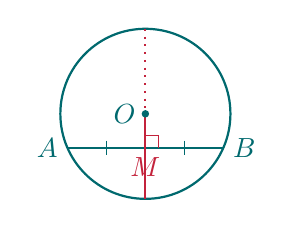
\begin{tikzpicture}[scale=0.9]
    \draw[thick, color=brandNavy] (0,0) circle (1.2);
    \coordinate (O) at (0,0);
    \coordinate (A) at (-1.1,-0.48);
    \coordinate (B) at (1.1,-0.48);
    \coordinate (M) at (0,-0.48);
    \draw[thick, color=brandNavy] (A) -- (B);
    \draw[thick, dotted, color=brandCrimson] (0,1.2) -- (0,0);
    \draw[thick, color=brandCrimson] (0,0) -- (0,-1.2);
    \fill[brandNavy] (O) circle (1.5pt) node[left] {$O$};
    \node[left, color=brandNavy] at (A) {$A$};
    \node[right, color=brandNavy] at (B) {$B$};
    \node[below, color=brandCrimson] at (M) {$M$};
    \draw[color=brandCrimson] (0,-0.3) -| (0.18,-0.48);
    \draw[color=brandNavy] (-0.55,-0.38) -- (-0.55,-0.58);
    \draw[color=brandNavy] (0.55,-0.38) -- (0.55,-0.58);
  \end{tikzpicture}
\end{minipage}
\end{khcard}

\vspace{6pt}
\setlength{\columnsep}{20pt}
\setlength{\columnseprule}{0.5pt}
\def\columnseprulecolor{\color{koreaTeal!40}}

\begin{multicols}{2}
  \noindent
  \exhead{1} គេមានរង្វង់ផ្ចិត $O$ និងអង្កត់ធ្នូ $AB = 10\text{cm}$ ( ដូចរូប) ។ បើ $OC$ កែងទៅនឹង $AB$ ចូរគណនាប្រវែង $AC$ ៖
  \begin{center}
    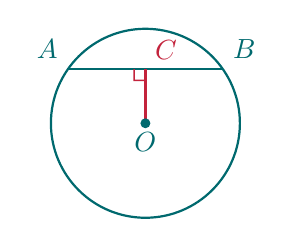
\begin{tikzpicture}[scale=1.2]
      \draw[thick, color=brandNavy] (0,0) circle (1.0);
      \coordinate (O) at (0,0);
      \coordinate (A) at (145:1.0);
      \coordinate (B) at (35:1.0);
      \coordinate (C) at ($(A)!0.5!(B)$);
      \draw[thick, color=brandNavy] (A) node[above left] {$A$} -- (B) node[above right] {$B$};
      \draw[thick, color=brandCrimson] (O) -- (C);
      \node[above right, color=brandCrimson] at (C) {$C$};
      \fill[brandNavy] (O) circle (1.5pt) node[below] {$O$};
      \draw[color=brandCrimson, line width=0.5pt] ($(C)!0.12cm!(A)$) -- ($($(C)!0.12cm!(A)$)+($(C)!0.12cm!(O)$)-(C)$) -- ($(C)!0.12cm!(O)$);
    \end{tikzpicture}
  \end{center}

  \vspace{2pt}
  \noindent
  \exhead{2} គេមានរង្វង់ផ្ចិត $O$ ( ដូចរូប) ដែលមាន $OM = 5\text{cm}$ និង $OB = 7\text{cm}$ ចូរគណនាប្រវែងអង្កត់ធ្នូ $AB$ ៖
  \begin{center}
    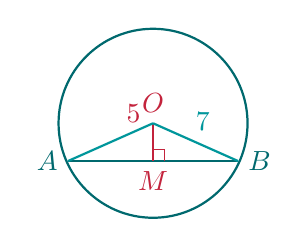
\begin{tikzpicture}[scale=1.2]
      \draw[thick, color=brandNavy] (0,0) circle (1.0);
      \coordinate (O) at (0,0);
      \coordinate (A) at (-0.9,-0.40);
      \coordinate (B) at (0.9,-0.40);
      \coordinate (M) at (0,-0.40);
      \draw[thick, color=brandNavy] (A) node[left] {$A$} -- (B) node[right] {$B$};
      \draw[thick, color=brandCrimson] (O) node[above] {$O$} -- (M) node[below] {$M$};
      \draw[thick, color=brandBlue] (O) -- (A);
      \draw[thick, color=brandBlue] (O) -- (B);
      \draw[color=brandCrimson, line width=0.5pt] ($(M)!0.12cm!(B)$) -- ($($(M)!0.12cm!(B)$)+($(M)!0.12cm!(O)$)-(M)$) -- ($(M)!0.12cm!(O)$);
      \node[left, color=brandCrimson] at (-0.03,0.1) { $5$};
      \node[above right, color=brandBlue] at (0.35,-0.18) { $7$};
    \end{tikzpicture}
  \end{center}

  \vspace{2pt}
  \noindent
  \exhead{3} នៅក្នុងរង្វង់ផ្ចិត $O$ គេមាន $\angle OXY = 30^\circ, \angle XOY = 60^\circ$ និង $XZ = 32\text{cm}$ ចូរគណនារង្វាស់ $XY$ ៖
  \begin{center}
    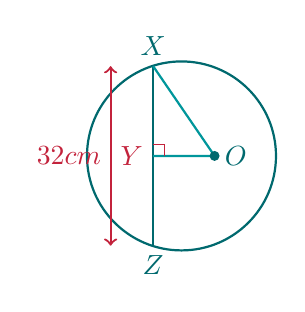
\begin{tikzpicture}[scale=1.2]
      \draw[thick, color=brandNavy] (0,0) circle (1.0);
      \coordinate (O) at (0.35,0);
      \coordinate (X) at (-0.3, 0.95);
      \coordinate (Z) at (-0.3, -0.95);
      \coordinate (Y) at (-0.3, 0);
      \draw[thick, color=brandNavy] (X) node[above] {$X$} -- (Z) node[below] {$Z$};
      \draw[thick, color=brandBlue] (X) -- (O) node[right, color=brandNavy] {$O$} -- (Y) node[left, color=brandCrimson] {$Y$};
      \fill[brandNavy] (O) circle (1.5pt);
      \draw[color=brandCrimson, line width=0.5pt] ($(Y)!0.12cm!(X)$) -- ($($(Y)!0.12cm!(X)$)+($(Y)!0.12cm!(O)$)-(Y)$) -- ($(Y)!0.12cm!(O)$);
      \draw[<->, thick, color=brandCrimson] (-0.75, 0.95) -- (-0.75, -0.95);
      \node[left, color=brandCrimson] at (-0.75, 0) { $32\text{cm}$};
    \end{tikzpicture}
  \end{center}

  \columnbreak

  \noindent
  \exhead{4} គេមាន $O$ ជាផ្ចិតនៃរង្វង់ $AB = 25\text{cm}$ និង $BQ = 6.5\text{cm}$ ដូចរូបខាងស្ដាំនេះ ៖
  \begin{center}
    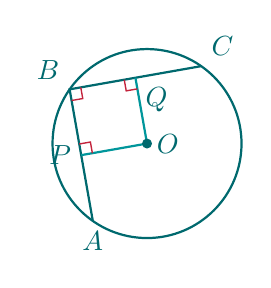
\begin{tikzpicture}[scale=1.2]
      \draw[thick, color=brandNavy] (0,0) circle (1.0);
      \coordinate (O) at (0,0);
      \coordinate (B) at (145:1.0);
      \coordinate (A) at (235:1.0);
      \coordinate (C) at (55:1.0);
      \coordinate (P) at ($(A)!0.5!(B)$);
      \coordinate (Q) at ($(B)!0.5!(C)$);
      \draw[thick, color=brandNavy] (A) node[below] {$A$} -- (B) node[above left] {$B$} -- (C) node[above right] {$C$};
      \draw[thick, color=brandTeal] (O) -- (P) node[left, color=brandNavy] {$P$};
      \draw[thick, color=brandTeal] (O) -- (Q) node[below right, color=brandNavy] {$Q$};
      \fill[brandNavy] (O) circle (1.5pt) node[right] {$O$};
      % Right angle at B (AB perpendicular to BC)
      \draw[color=brandCrimson, line width=0.5pt] ($(B)!0.12cm!(A)$) -- ($($(B)!0.12cm!(A)$)+($(B)!0.12cm!(C)$)-(B)$) -- ($(B)!0.12cm!(C)$);
      % Right angle at P (OP perpendicular to AB)
      \draw[color=brandCrimson, line width=0.5pt] ($(P)!0.12cm!(B)$) -- ($($(P)!0.12cm!(B)$)+($(P)!0.12cm!(O)$)-(P)$) -- ($(P)!0.12cm!(O)$);
      % Right angle at Q (OQ perpendicular to BC)
      \draw[color=brandCrimson, line width=0.5pt] ($(Q)!0.12cm!(B)$) -- ($($(Q)!0.12cm!(B)$)+($(Q)!0.12cm!(O)$)-(Q)$) -- ($(Q)!0.12cm!(O)$);
    \end{tikzpicture}
  \end{center}

  \vspace{2pt}
  \noindent
  \exhead{5} គេមានរង្វង់ផ្ចិត $O$ មានកាំ $r = 10\text{cm}$ និងអង្កត់ធ្នូ $CD = 16\text{cm}$ (ដូចរូប) ។ បើ $OH \perp CD$ ត្រង់ $H$ ចូរគណនាចម្ងាយ $OH$ ៖
  \begin{center}
    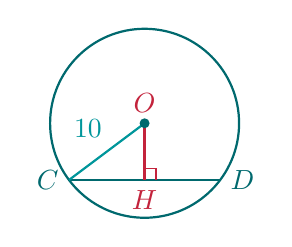
\begin{tikzpicture}[scale=1.2]
      \draw[thick, color=brandNavy] (0,0) circle (1.0);
      \coordinate (O) at (0,0);
      \coordinate (C) at (-0.8,-0.6);
      \coordinate (D) at (0.8,-0.6);
      \coordinate (H) at (0,-0.6);
      \draw[thick, color=brandNavy] (C) node[left] {$C$} -- (D) node[right] {$D$};
      \draw[thick, color=brandCrimson] (O) node[above] {$O$} -- (H) node[below] {$H$};
      \draw[thick, color=brandBlue] (O) -- (C);
      \draw[color=brandCrimson, line width=0.5pt] ($(H)!0.12cm!(D)$) -- ($($(H)!0.12cm!(D)$)+($(H)!0.12cm!(O)$)-(H)$) -- ($(H)!0.12cm!(O)$);
      \fill[brandNavy] (O) circle (1.5pt);
      \node[above left, color=brandBlue] at (-0.35,-0.25) {$10$};
    \end{tikzpicture}
  \end{center}

  \vspace{2pt}
  \noindent
  \exhead{6} ក្នុងរង្វង់ផ្ចិត $O$ គេមានអង្កត់ផ្ចិត $AB = 20\text{cm}$ និងអង្កត់ធ្នូ $MN \perp AB$ ត្រង់ $I$ (ដូចរូប) ។ បើ $OI = 6\text{cm}$ ចូរគណនាប្រវែង $MN$ ៖
  \begin{center}
    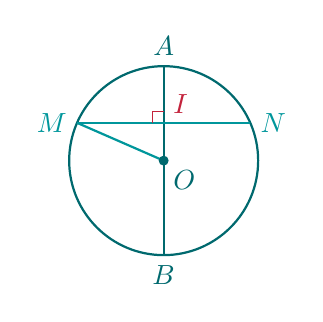
\begin{tikzpicture}[scale=1.2]
      \draw[thick, color=brandNavy] (0,0) circle (1.0);
      \coordinate (O) at (0,0);
      \coordinate (A) at (0, 1.0);
      \coordinate (B) at (0, -1.0);
      \coordinate (I) at (0, 0.4);
      \coordinate (M) at (-0.916, 0.4);
      \coordinate (N) at (0.916, 0.4);
      \draw[thick, color=brandNavy] (A) node[above] {$A$} -- (B) node[below] {$B$};
      \draw[thick, color=brandTeal] (M) node[left] {$M$} -- (N) node[right] {$N$};
      \draw[thick, color=brandBlue] (O) -- (M);
      \fill[brandNavy] (O) circle (1.5pt) node[below right] {$O$};
      \node[above right, color=brandCrimson] at (I) { $I$};
      \draw[color=brandCrimson, line width=0.5pt] ($(I)!0.12cm!(M)$) -- ($($(I)!0.12cm!(M)$)+($(I)!0.12cm!(A)$)-(I)$) -- ($(I)!0.12cm!(A)$);
    \end{tikzpicture}
  \end{center}
\end{multicols}

\newpage
% -------------------------------------------------------------------------
% SECTION 1.2

\khsubsection{១.២}{អង្កត់ធ្នូស្មើគ្នា}

\begin{khboxorange}
  \begin{minipage}[c]{0.72\textwidth}
    \begin{itemize}[leftmargin=12pt, itemsep=1.5pt, topsep=0pt, parsep=0pt]
      \item[\color{brandNavy}\ding{228}] អង្កត់ធ្នូពីរមានប្រវែងស្មើគ្នាក្នុងរង្វង់មួយ ត្រូវមានចម្ងាយស្មើគ្នាពីផ្ចិតនៃរង្វង់នោះ ។
      \item[\color{brandNavy}\ding{228}] ច្រាសមកវិញ ៖ អង្កត់ធ្នូក្នុងរង្វង់មួយដែលមានចម្ងាយស្មើគ្នាពីផ្ចិតនៃរង្វង់ ជាអង្កត់ធ្នូប៉ុនគ្នា ។
    \end{itemize}
  \end{minipage}\hfill
  \begin{minipage}[c]{0.25\textwidth}
    \centering
    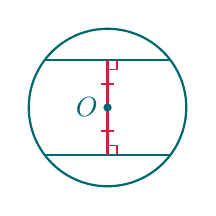
\begin{tikzpicture}[scale=1]
      \draw[thick, color=brandNavy] (0,0) circle (1.0);
      \coordinate (O) at (0,0);
      \coordinate (M1) at (0, 0.60);
      \coordinate (M2) at (0, -0.60);
      \draw[thick, color=brandNavy] (-0.80, 0.60) -- (0.80, 0.60);
      \draw[thick, color=brandNavy] (-0.80, -0.60) -- (0.80, -0.60);
      \draw[thick, color=brandCrimson] (O) -- (M1);
      \draw[thick, color=brandCrimson] (O) -- (M2);
      \fill[brandNavy] (O) circle (1.5pt) node[left] { $O$};
      \draw[color=brandCrimson, line width=0.5pt] (0, 0.48) -| (0.12, 0.60);
      \draw[color=brandCrimson, line width=0.5pt] (0, -0.48) -| (0.12, -0.60);
      \draw[thick, color=brandCrimson] (-0.08, 0.30) -- (0.08, 0.30);
      \draw[thick, color=brandCrimson] (-0.08, -0.30) -- (0.08, -0.30);
    \end{tikzpicture}
  \end{minipage}
\end{khboxorange}

\vspace{4pt}
\begin{multicols}{2}
  % Exercise 07
  \noindent
  \exhead{7} គេមានរង្វង់ផ្ចិត $O$ ដែលមានកាំ $5\text{cm}$ និងអង្កត់ធ្នូ $AB$ ប្រវែង $8\text{cm}$ ៖ បើ $OM \perp AB$ ត្រង់ $M$ ៖ រកចម្ងាយ $OM$ ពីផ្ចិតរង្វង់ទៅអង្កត់ធ្នូ ៖\par
  \vspace{1pt}
  {\centering
    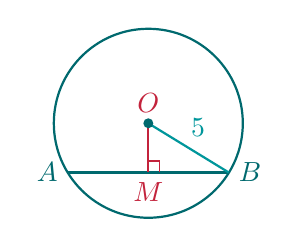
\begin{tikzpicture}[scale=1.2]
      \draw[thick, color=brandNavy] (0,0) circle (1.0);
      \coordinate (O) at (0,0);
      \coordinate (A) at (-0.85,-0.52);
      \coordinate (B) at (0.85,-0.52);
      \coordinate (M) at (0,-0.52);
      \draw[thick, color=brandNavy] (A) node[left] {$A$} -- (B) node[right] {$B$};
      \draw[thick, color=brandCrimson] (O) node[above] {$O$} -- (M) node[below] {$M$};
      \draw[thick, color=brandBlue] (O) -- (B);
      \fill[brandNavy] (O) circle (1.5pt);
      \draw[color=brandCrimson, line width=0.5pt] ($(M)!0.12cm!(B)$) -- ($($(M)!0.12cm!(B)$)+($(M)!0.12cm!(O)$)-(M)$) -- ($(M)!0.12cm!(O)$);
      \node[above right, color=brandBlue] at (0.35,-0.24) { $5$};
    \end{tikzpicture}\par}

  \vspace{3pt}
  % Exercise 08
  \noindent
  \exhead{8} ក្នុងរូបខាងក្រោមនេះ $O$ ជាផ្ចិតនៃរង្វង់ដែលមានកាំ $5\text{cm}$ ហើយ $PQ = RS = 6\text{cm}$ ៖ រកប្រវែង $OX$ និង $OY$ ៖\par
  \vspace{1pt}
  {\centering
    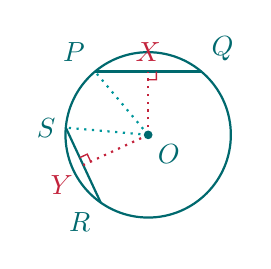
\begin{tikzpicture}[scale=1.05]
      \draw[thick, color=brandNavy] (0,0) circle (1.0);
      \coordinate (O) at (0,0);
      \coordinate (P) at (130:1.0);
      \coordinate (Q) at (50:1.0);
      \coordinate (S) at (175:1.0);
      \coordinate (R) at (235:1.0);
      \coordinate (X) at ($(P)!0.5!(Q)$);
      \coordinate (Y) at ($(R)!0.5!(S)$);
      \draw[thick, color=brandNavy] (P) node[above left] {$P$} -- (Q) node[above right] {$Q$};
      \draw[thick, color=brandNavy] (S) node[left] {$S$} -- (R) node[below left] {$R$};
      \draw[thick, dotted, color=brandCrimson] (O) -- (X) node[above] {$X$};
      \draw[thick, dotted, color=brandCrimson] (O) -- (Y) node[below left, color=brandCrimson] {$Y$};
      \draw[thick, dotted, color=brandBlue] (O) -- (P);
      \draw[thick, dotted, color=brandBlue] (O) -- (S);
      \fill[brandNavy] (O) circle (1.5pt) node[below right] {$O$};
      \draw[color=brandCrimson, line width=0.5pt] ($(X)!0.10cm!(Q)$) -- ($($(X)!0.10cm!(Q)$)+($(X)!0.10cm!(O)$)-(X)$) -- ($(X)!0.10cm!(O)$);
      \draw[color=brandCrimson, line width=0.5pt] ($(Y)!0.10cm!(S)$) -- ($($(Y)!0.10cm!(S)$)+($(Y)!0.10cm!(O)$)-(Y)$) -- ($(Y)!0.10cm!(O)$);
    \end{tikzpicture}\par}

  \vspace{3pt}
  % Exercise 09
  \noindent
  \exhead{9} គេមានរង្វង់ផ្ចិត $O$ ដែលមានកាំ $10\text{cm}$ ហើយ $PR = QS$ និង $OC = 5\text{cm}$ ៖ រកប្រវែង $OD$ និង $PR$ ។(ណែនាំ៖គូស $OR$) \par
  \vspace{1pt}
  {\centering
    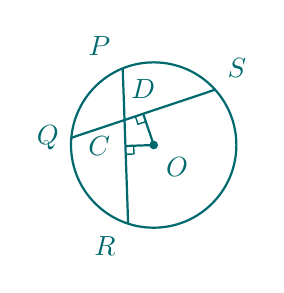
\begin{tikzpicture}[scale=1.05]
      \draw[thick, color=brandNavy] (0,0) circle (1.0);
      \coordinate (O) at (0,0);
      \coordinate (P) at (112:1.0);
      \coordinate (R) at (252:1.0);
      \coordinate (Q) at (175:1.0);
      \coordinate (S) at (42:1.0);
      \coordinate (C) at ($(P)!(O)!(R)$);
      \coordinate (D) at ($(Q)!(O)!(S)$);
      \draw[thick, color=brandNavy] (P) -- (R);
      \draw[thick, color=brandNavy] (Q) -- (S);
      \draw[thick, color=brandNavy] (O) -- (C);
      \draw[thick, color=brandNavy] (O) -- (D);
      \fill[brandNavy] (O) circle (1.5pt) node[below right=1pt] {$O$};
      \node[above left=1pt, color=brandNavy] at (P) {$P$};
      \node[below left=1pt, color=brandNavy] at (R) {$R$};
      \node[left=1pt, color=brandNavy] at (Q) {$Q$};
      \node[above right=1pt, color=brandNavy] at (S) {$S$};
      \node[left=2pt, color=brandNavy] at (C) {$C$};
      \node[above=2pt, color=brandNavy] at (D) {$D$};
      \draw[color=brandNavy, line width=0.5pt] ($(C)!0.10cm!(R)$) -- ($($(C)!0.10cm!(R)$)+($(C)!0.10cm!(O)$)-(C)$) -- ($(C)!0.10cm!(O)$);
      \draw[color=brandNavy, line width=0.5pt] ($(D)!0.10cm!(Q)$) -- ($($(D)!0.10cm!(Q)$)+($(D)!0.10cm!(O)$)-(D)$) -- ($(D)!0.10cm!(O)$);
    \end{tikzpicture}\par}

  \vspace{3pt}
  % Exercise 10
  \noindent
  \exhead{10} ក្នុងរូបខាងក្រោមនេះគេមាន $O$ ជាផ្ចិតនៃរង្វង់ហើយ $OA = OB = 5.5\text{cm}$ និង $MN = 9\text{cm}$ ៖ រកប្រវែង $NP$ ៖\par
  \vspace{1pt}
  {\centering
    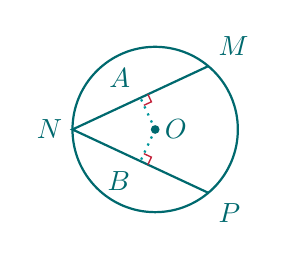
\begin{tikzpicture}[scale=1.05]
      \draw[thick, color=brandNavy] (0,0) circle (1.0);
      \coordinate (O) at (0,0);
      \coordinate (N) at (180:1.0);
      \coordinate (M) at (50:1.0);
      \coordinate (P) at (-50:1.0);
      \coordinate (A) at ($(M)!0.5!(N)$);
      \coordinate (B) at ($(N)!0.5!(P)$);
      \draw[thick, color=brandNavy] (M) node[above right] {$M$} -- (N) node[left] {$N$} -- (P) node[below right] {$P$};
      \draw[thick, dotted, color=brandTeal] (O) -- (A) node[above left, color=brandNavy] {$A$};
      \draw[thick, dotted, color=brandTeal] (O) -- (B) node[below left, color=brandNavy] {$B$};
      \fill[brandNavy] (O) circle (1.5pt) node[right] {$O$};
      \draw[color=brandCrimson, line width=0.5pt] ($(A)!0.10cm!(M)$) -- ($($(A)!0.10cm!(M)$)+($(A)!0.10cm!(O)$)-(A)$) -- ($(A)!0.10cm!(O)$);
      \draw[color=brandCrimson, line width=0.5pt] ($(B)!0.10cm!(P)$) -- ($($(B)!0.10cm!(P)$)+($(B)!0.10cm!(O)$)-(B)$) -- ($(B)!0.10cm!(O)$);
    \end{tikzpicture}\par}

  \columnbreak

  % Exercise 11
  \noindent
  \exhead{11} ក្នុងរង្វង់ផ្ចិត $O$ មានកាំ $r = 13\text{cm}$ គេមាន $AB = CD$ ៖ បើ $OH \perp AB$ ត្រង់ $H$, $OH = 5\text{cm}$ និង $OK \perp CD$ ត្រង់ $K$ ៖ គណនាប្រវែង $AH, AB$ និងចម្ងាយ $OK$ ៖\par
  \vspace{1pt}
  {\centering
    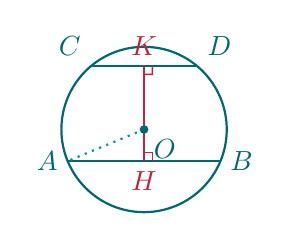
\begin{tikzpicture}[scale=1.05]
      \draw[thick, color=brandNavy] (0,0) circle (1.0);
      \coordinate (O) at (0,0);
      \coordinate (A) at (-0.92,-0.38);
      \coordinate (B) at (0.92,-0.38);
      \coordinate (H) at (0,-0.38);
      \coordinate (C) at (130:1.0);
      \coordinate (D) at (50:1.0);
      \coordinate (K) at ($(C)!0.5!(D)$);
      \draw[thick, color=brandNavy] (A) node[left] {$A$} -- (B) node[right] {$B$};
      \draw[thick, color=brandNavy] (C) node[above left] {$C$} -- (D) node[above right] {$D$};
      \draw[thick, color=brandCrimson] (O) -- (H) node[below, color=brandCrimson] {$H$};
      \draw[thick, color=brandCrimson] (O) -- (K) node[above, color=brandCrimson] {$K$};
      \draw[thick, dotted, color=brandBlue] (O) -- (A);
      \fill[brandNavy] (O) circle (1.5pt) node[below right] {$O$};
      \draw[color=brandCrimson, line width=0.5pt] ($(H)!0.10cm!(B)$) -- ($($(H)!0.10cm!(B)$)+($(H)!0.10cm!(O)$)-(H)$) -- ($(H)!0.10cm!(O)$);
      \draw[color=brandCrimson, line width=0.5pt] ($(K)!0.10cm!(D)$) -- ($($(K)!0.10cm!(D)$)+($(K)!0.10cm!(O)$)-(K)$) -- ($(K)!0.10cm!(O)$);
    \end{tikzpicture}\par}

  \vspace{3pt}
  % Exercise 12
  \noindent
  \exhead{12} ក្នុងរង្វង់ផ្ចិត $O$ គេមានអង្កត់ធ្នូពីរ $AB = 8\text{cm}$ និង $CD = 6\text{cm}$ ដែលស្របគ្នា ៖ បើកាំរង្វង់ $r = 5\text{cm}$ ៖ គណនាចម្ងាយរវាងអង្កត់ធ្នូទាំងពីរ $AB$ និង $CD$ (ករណីអង្កត់ធ្នូទាំងពីរនៅសងខាងផ្ចិត $O$) ៖\par
  \vspace{1pt}
  {\centering
    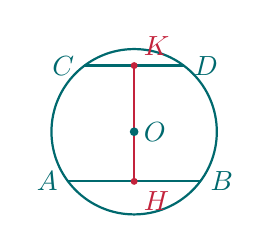
\begin{tikzpicture}[scale=1.05]
      \draw[thick, color=brandNavy] (0,0) circle (1.0);
      \coordinate (O) at (0,0);
      \coordinate (A) at (-0.8,-0.6);
      \coordinate (B) at (0.8,-0.6);
      \coordinate (C) at (-0.6,0.8);
      \coordinate (D) at (0.6,0.8);
      \coordinate (H) at (0,-0.6);
      \coordinate (K) at (0,0.8);
      \draw[thick, color=brandNavy] (A) node[left] {$A$} -- (B) node[right] {$B$};
      \draw[thick, color=brandNavy] (C) node[left] {$C$} -- (D) node[right] {$D$};
      \draw[thick, color=brandCrimson] (K) -- (H);
      \fill[brandNavy] (O) circle (1.5pt) node[right] {$O$};
      \fill[brandCrimson] (H) circle (1.2pt) node[below right] {$H$};
      \fill[brandCrimson] (K) circle (1.2pt) node[above right] {$K$};
    \end{tikzpicture}\par}

  \vspace{3pt}
  % Exercise 13
  \noindent
  \exhead{13} ដូចលំហាត់ទី ១២ ដែរ ប៉ុន្តែករណីអង្កត់ធ្នូទាំងពីរ $AB$ និង $CD$ នៅខាងតែមួយនៃផ្ចិត $O$ ៖ គណនាចម្ងាយរវាងអង្កត់ធ្នូទាំងពីរ ៖\par
  \vspace{1pt}
  {\centering
    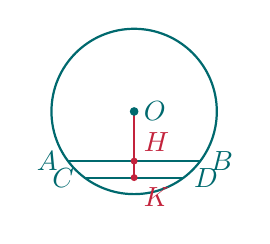
\begin{tikzpicture}[scale=1.05]
      \draw[thick, color=brandNavy] (0,0) circle (1.0);
      \coordinate (O) at (0,0);
      \coordinate (A) at (-0.8,-0.6);
      \coordinate (B) at (0.8,-0.6);
      \coordinate (C) at (-0.6,-0.8);
      \coordinate (D) at (0.6,-0.8);
      \coordinate (H) at (0,-0.6);
      \coordinate (K) at (0,-0.8);
      \draw[thick, color=brandNavy] (A) node[left] {$A$} -- (B) node[right] {$B$};
      \draw[thick, color=brandNavy] (C) node[left] {$C$} -- (D) node[right] {$D$};
      \draw[thick, color=brandCrimson] (O) -- (K);
      \fill[brandNavy] (O) circle (1.5pt) node[right] {$O$};
      \fill[brandCrimson] (H) circle (1.2pt) node[above right] {$H$};
      \fill[brandCrimson] (K) circle (1.2pt) node[below right] {$K$};
    \end{tikzpicture}\par}

  \vspace{3pt}
  % Exercise 14
  \noindent
  \exhead{14} ក្នុងរង្វង់ផ្ចិត $O$ គេមានអង្កត់ធ្នូ $AB = 12\text{cm}$ និង $CD = 16\text{cm}$ ស្របគ្នា ៖ បើចម្ងាយរវាងអង្កត់ធ្នូទាំងពីរស្មើនឹង $14\text{cm}$ ៖ គណនាកាំ $r$ នៃរង្វង់ ៖\par
  \vspace{1pt}
  {\centering
    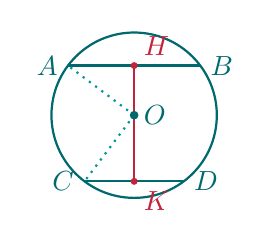
\begin{tikzpicture}[scale=1.05]
      \draw[thick, color=brandNavy] (0,0) circle (1.0);
      \coordinate (O) at (0,0);
      \coordinate (A) at (-0.8,0.6);
      \coordinate (B) at (0.8,0.6);
      \coordinate (C) at (-0.6,-0.8);
      \coordinate (D) at (0.6,-0.8);
      \coordinate (H) at (0,0.6);
      \coordinate (K) at (0,-0.8);
      \draw[thick, color=brandNavy] (A) node[left] {$A$} -- (B) node[right] {$B$};
      \draw[thick, color=brandNavy] (C) node[left] {$C$} -- (D) node[right] {$D$};
      \draw[thick, color=brandCrimson] (H) -- (K);
      \draw[thick, dotted, color=brandBlue] (O) -- (A);
      \draw[thick, dotted, color=brandBlue] (O) -- (C);
      \fill[brandNavy] (O) circle (1.5pt) node[right] {$O$};
      \fill[brandCrimson] (H) circle (1.2pt) node[above right] {$H$};
      \fill[brandCrimson] (K) circle (1.2pt) node[below right] {$K$};
    \end{tikzpicture}\par}

\end{multicols}

\vspace{7pt}
\newpage
% -------------------------------------------------------------------------
% SECTION 2 (LINE TANGENT TO CIRCLE)
\khsection{២}{បន្ទាត់ប៉ះរង្វង់}

\begin{khboxmagenta}
  \textbf{បន្ទាត់ប៉ះរង្វង់គឺជាបន្ទាត់ដែលមានចំណុចរួមតែមួយជាមួយរង្វង់ ហើយកែងទៅនឹងកាំត្រង់ចំណុចប៉ះនោះ ។}
\end{khboxmagenta}

\vspace{3pt}
\noindent
\exhead{15} ក្នុងរូបខាងក្រោម $PT$ ជាបន្ទាត់ប៉ះរង្វង់ផ្ចិត $O$ ត្រង់ $T$ ៖

\vspace{2pt}
\begin{multicols}{2}
  % Sub-card ក
  \noindent
  \begin{khcard}[equal height group=ex15cards]
    \alphabadge{ក} ចូររកតម្លៃនៃមុំ $a$\\[1pt]
    {\centering
      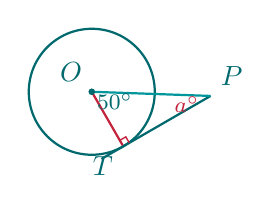
\begin{tikzpicture}[scale=0.8]
        \draw[thick, color=brandNavy] (0,0) circle (1.0);
        \coordinate (O) at (0,0);
        \coordinate (T) at (-60:1.0);
        \coordinate (P) at ($(T) + (30:1.6)$);
        \draw[thick, color=brandCrimson] (O) -- (T) node[below left, color=brandNavy] {$T$};
        \draw[thick, color=brandNavy] ($(T)+(-150:0.4)$) -- (P) node[above right] {$P$};
        \draw[thick, color=brandBlue] (O) -- (P);
        \fill[brandNavy] (O) circle (1.5pt) node[above left] {$O$};
        \draw[color=brandCrimson, line width=0.5pt] ($(T)!0.11cm!(P)$) -- ($($(T)!0.11cm!(P)$)+($(T)!0.11cm!(O)$)-(T)$) -- ($(T)!0.11cm!(O)$);
        \node[color=brandNavy] at (-23:0.4) {\footnotesize $50^\circ$};
        \node[color=brandCrimson] at ($(P)+(-160:0.4)$) {\footnotesize $a^\circ$};
      \end{tikzpicture}\par}
  \end{khcard}

  \vspace{3pt}
  % Sub-card ខ
  \noindent
  \begin{khcard}[equal height group=ex15cards]
    \alphabadge{ខ} ចូររកតម្លៃនៃមុំ $a$ និង $b$\\[1pt]
    {\centering
      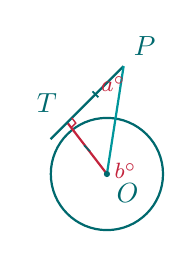
\begin{tikzpicture}[scale=0.75]
        \draw[thick, color=brandNavy] (0,-0.2) circle (0.95);
        \coordinate (O) at (0,-0.2);
        \coordinate (T) at (135:0.95);
        \coordinate (P) at ($(T) + (45:1.35)$);
        \draw[thick, color=brandCrimson] (O) -- (T) node[above left, color=brandNavy] {$T$};
        \draw[thick, color=brandNavy] ($(T)+(-135:0.4)$) -- (P) node[above right] {$P$};
        \draw[thick, color=brandBlue] (O) -- (P);
        \fill[brandNavy] (O) circle (1.5pt) node[below right] {$O$};
        \draw[color=brandCrimson, line width=0.5pt] ($(T)!0.11cm!(P)$) -- ($($(T)!0.11cm!(P)$)+($(T)!0.11cm!(O)$)-(T)$) -- ($(T)!0.11cm!(O)$);
        \draw[color=brandNavy, line width=0.6pt] ($(T)!0.5!(P)+(-0.05,0.05)$) -- ($(T)!0.5!(P)+(0.05,-0.05)$);
        \draw[color=brandNavy, line width=0.6pt] ($(O)!0.5!(T)+(-0.05,0.05)$) -- ($(O)!0.5!(T)+(0.05,-0.05)$);
        \node[color=brandCrimson] at ($(P)+(-120:0.35)$) {\footnotesize $a^\circ$};
        \node[color=brandCrimson] at ($(O)+(9:0.32)$) {\footnotesize $b^\circ$};
      \end{tikzpicture}\par}
  \end{khcard}

  \vspace{3pt}
  % Sub-card គ
  \noindent
  \begin{khcard}[equal height group=ex15cards]
    \alphabadge{គ} ចូររកតម្លៃនៃមុំ $b$\\[1pt]
    {\centering
      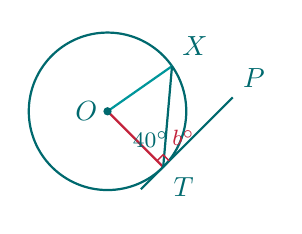
\begin{tikzpicture}[scale=1]
        \draw[thick, color=brandNavy] (0,0) circle (1.0);
        \coordinate (O) at (0,0);
        \coordinate (T) at (-45:1.0);
        \coordinate (X) at (35:1.0);
        \coordinate (P) at ($(T) + (45:1.25)$);
        \draw[thick, color=brandCrimson] (O) node[left, color=brandNavy] {$O$} -- (T) node[below right, color=brandNavy] {$T$};
        \draw[thick, color=brandBlue] (O) -- (X) node[above right, color=brandNavy] {$X$};
        \draw[thick, color=brandNavy] (T) -- (X);
        \draw[thick, color=brandNavy] ($(T)+(-135:0.4)$) -- (P) node[above right] {$P$};
        \fill[brandNavy] (O) circle (1.5pt);
        \draw[color=brandCrimson, line width=0.5pt] ($(T)!0.11cm!(P)$) -- ($($(T)!0.11cm!(P)$)+($(T)!0.11cm!(O)$)-(T)$) -- ($(T)!0.11cm!(O)$);
        \node[color=brandNavy] at ($(T)+(115:0.38)$) {\footnotesize $40^\circ$};
        \node[color=brandCrimson] at ($(T)+(55:0.45)$) {\footnotesize $b^\circ$};
      \end{tikzpicture}\par}
  \end{khcard}

  \columnbreak

  % Sub-card ឃ
  \noindent
  \begin{khcard}[equal height group=ex15cards]
    \alphabadge{ឃ} ចូររកតម្លៃនៃមុំ $a$ និង $b$\\[1pt]
    {\centering
      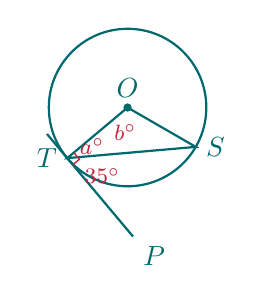
\begin{tikzpicture}[scale=1]
        \draw[thick, color=brandNavy] (0,0) circle (1.0);
        \coordinate (O) at (0,0);
        \coordinate (T) at (220:1.0);
        \coordinate (S) at (-30:1.0);
        \coordinate (P) at ($(T) + (-50:1.3)$);
        \draw[thick, color=brandNavy] (O) node[above] {$O$} -- (T) node[left] {$T$} -- (S) node[right] {$S$} -- cycle;
        \draw[thick, color=brandNavy] ($(T)+(130:0.4)$) -- (P) node[below right] {$P$};
        \fill[brandNavy] (O) circle (1.5pt);
        \draw[color=brandCrimson, line width=0.5pt] ($(T)!0.11cm!(P)$) -- ($($(T)!0.11cm!(P)$)+($(T)!0.11cm!(O)$)-(T)$) -- ($(T)!0.11cm!(O)$);
        \node[color=brandCrimson] at ($(O)+(-95:0.32)$) {\footnotesize $b^\circ$};
        \node[color=brandCrimson] at ($(T)+(25:0.35)$) {\footnotesize $a^\circ$};
        \node[color=brandCrimson] at ($(T)+(-27:0.5)$) {\footnotesize $35^\circ$};
      \end{tikzpicture}\par}
  \end{khcard}

  \vspace{3pt}
  % Sub-card ង
  \noindent
  \begin{khcard}[equal height group=ex15cards]
    \alphabadge{ង} ចូររកតម្លៃនៃមុំ $a, b$ និង $c$\\[1pt]
    {\centering
      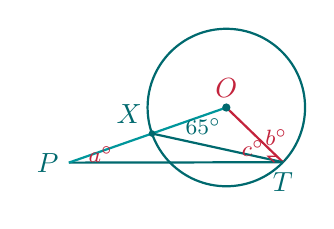
\begin{tikzpicture}[scale=1]
        \draw[thick, color=brandNavy] (0.5,0.4) circle (1.0);
        \coordinate (O) at (0.5,0.4);
        \coordinate (P) at (-1.5,-0.3);
        \coordinate (X) at ($(O)!1.0cm!(P)$);
        \coordinate (T) at ($(O)+(-44:1.0)$);
        
        \draw[thick, color=brandNavy] (P) node[left] {$P$} -- (T) node[below] {$T$};
        \draw[thick, color=brandCrimson] (O) node[above] {$O$} -- (T);
        \draw[thick, color=brandBlue] (P) -- (O);
        \draw[thick, color=brandNavy] (X) node[above left, color=brandNavy] {$X$} -- (T);
        \fill[brandNavy] (O) circle (1.5pt);
        \fill[brandNavy] (X) circle (1.2pt);
        
        \draw[color=brandCrimson, line width=0.5pt] ($(T)!0.11cm!(P)$) -- ($($(T)!0.11cm!(P)$)+($(T)!0.11cm!(O)$)-(T)$) -- ($(T)!0.11cm!(O)$);
        
        \node[color=brandCrimson] at ($(P)+(14:0.42)$) {\footnotesize $a^\circ$};
        \node[color=brandNavy] at ($(O)+(-140:0.38)$) {\footnotesize $65^\circ$};
        \node[color=brandCrimson] at ($(T)+(105:0.32)$) {\footnotesize $b^\circ$};
        \node[color=brandCrimson] at ($(T)+(155:0.42)$) {\footnotesize $c^\circ$};
      \end{tikzpicture}\par}
  \end{khcard}

  \vspace{3pt}
  % Sub-card ច
  \noindent
  \begin{khcard}[equal height group=ex15cards]
    \alphabadge{ច} $AOT$ និង $BOP$ ជាបន្ទាត់ត្រង់ ៖ ចូររកមុំ $a, b$\\[1pt]
    {\centering
      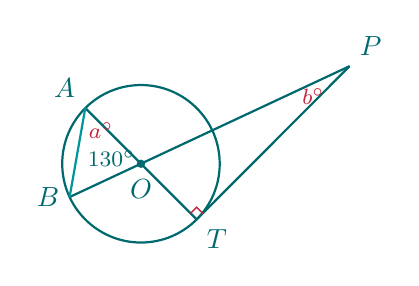
\begin{tikzpicture}[scale=1]
        \draw[thick, color=brandNavy] (0,0) circle (1.0);
        \coordinate (O) at (0,0);
        \coordinate (A) at (135:1.0);
        \coordinate (T) at (-45:1.0);
        \coordinate (B) at (205:1.0);
        \coordinate (P) at (2.65, 1.24);
        
        \draw[thick, color=brandNavy] (A) node[above left] {$A$} -- (T) node[below right] {$T$};
        \draw[thick, color=brandNavy] (B) node[left] {$B$} -- (P) node[above right] {$P$};
        \draw[thick, color=brandBlue] (A) -- (B);
        \draw[thick, color=brandNavy] (T) -- (P);
        \fill[brandNavy] (O) circle (1.5pt) node[below=2pt] {$O$};
        
        \draw[color=brandCrimson, line width=0.5pt] ($(T)!0.11cm!(P)$) -- ($($(T)!0.11cm!(P)$)+($(T)!0.11cm!(O)$)-(T)$) -- ($(T)!0.11cm!(O)$);
        
        \node[color=brandNavy] at ($(O)+(170:0.38)$) {\footnotesize $130^\circ$};
        \node[color=brandCrimson] at ($(A)+(-55:0.35)$) {\footnotesize $a^\circ$};
        \node[color=brandCrimson] at ($(P)+(-140:0.60)$) {\footnotesize $b^\circ$};
      \end{tikzpicture}\par}
  \end{khcard}
\end{multicols}

\vspace{3pt}
\noindent
\begin{minipage}[c]{0.64\textwidth}
  \exhead{16} គេមានរង្វង់មួយដែលមានផ្ចិត $O$ និងកាំស្មើនឹង $2\text{cm}$ ៖ $A$ ជាចំណុចមួយនៅក្រៅរង្វង់។ ពីចំណុច $A$ គេគូសបន្ទាត់ប៉ះនឹងរង្វង់ត្រង់ចំណុច $B$ និងបន្ទាត់មួយទៀត $AC$ កាត់តាមផ្ចិត $O$ និងកាត់រង្វង់ត្រង់ $C$ ៖
  \begin{itemize}[leftmargin=15pt, itemsep=0.5pt]
    \item[\alphabadge{ក}] បង្ហាញថា $\Delta ABO$ ជាត្រីកោណកែងត្រង់ $B$ ៖\\
      {\footnotesize\color{brandCrimson}\textit{(ណែនាំ៖ បន្ទាត់ប៉ះរង្វង់តែងតែកែងទៅនឹងកាំត្រង់ចំណុចប៉ះ $OB \perp AB$)}}
    \item[\alphabadge{ខ}] បើ $OA = 4\text{cm}$ ៖ គណនាប្រវែងបន្ទាត់ប៉ះ $AB$ ៖\\
      {\footnotesize\color{brandCrimson}\textit{(ណែនាំ៖ ប្រើទ្រឹស្តីបទពីតាករក្នុង $\Delta ABO \implies AB = \sqrt{OA^2 - OB^2}$)}}
  \end{itemize}
\end{minipage}\hfill
\begin{minipage}[c]{0.34\textwidth}
  \centering
  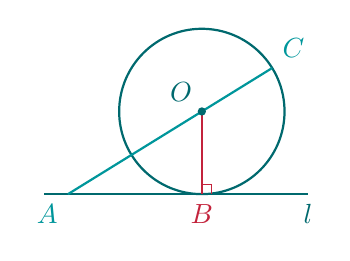
\begin{tikzpicture}[scale=1]
    \draw[thick, color=brandNavy] (0,0) circle (1.05);
    \coordinate (O) at (0,0);
    \coordinate (B) at (0,-1.05);
    \coordinate (A) at (-1.7,-1.05);
    \coordinate (C) at (31.7:1.05);
    \draw[thick, color=brandNavy] (-2.0,-1.05) -- (1.35,-1.05) node[below] {$l$};
    \draw[thick, color=brandCrimson] (O) -- (B) node[below] {$B$};
    \draw[thick, color=brandBlue] (A) node[below left] {$A$} -- (C) node[above right] {$C$};
    \fill[brandNavy] (O) circle (1.5pt) node[above left] {$O$};
    \draw[color=brandCrimson, line width=0.5pt] (0.12,-1.05) -- (0.12,-0.93) -- (0,-0.93);
  \end{tikzpicture}
\end{minipage}

\vspace{3pt}
\noindent
\begin{minipage}[c]{0.64\textwidth}
  \exhead{17} គេមានរង្វង់ផ្ចិត $O$ មានកាំ $r = 3\text{cm}$ និងចំណុច $P$ នៅក្រៅរង្វង់ ដែល $OP = 5\text{cm}$ ៖ ពីចំណុច $P$ គេគូសបន្ទាត់ប៉ះរង្វង់ត្រង់ $T$ និងបន្ទាត់កាត់ផ្ចិត $O$ ត្រង់ $A$ (ដូចរូប) ៖
  \begin{itemize}[leftmargin=15pt, itemsep=0.5pt]
    \item[\alphabadge{ក}] ស្រាយបំភ្លឺថា $OT \perp PT$ ត្រង់ចំណុចប៉ះ $T$ ៖\\
      {\footnotesize\color{brandCrimson}\textit{(ណែនាំ៖ តាមលក្ខណៈបន្ទាត់ប៉ះរង្វង់ $PT$ កែងនឹងកាំ $OT$ ត្រង់ចំណុចប៉ះ $T$)}}
    \item[\alphabadge{ខ}] គណនាប្រវែងបន្ទាត់ប៉ះ $PT$ ៖\\
      {\footnotesize\color{brandCrimson}\textit{(ណែនាំ៖ អនុវត្តទ្រឹស្តីបទពីតាករក្នុង $\Delta PTO \implies PT = \sqrt{OP^2 - OT^2}$)}}
  \end{itemize}
\end{minipage}\hfill
\begin{minipage}[c]{0.34\textwidth}
  \centering
  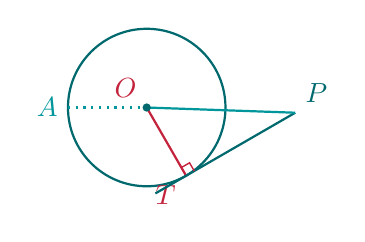
\begin{tikzpicture}[scale=1]
    \draw[thick, color=brandNavy] (0,0) circle (1.0);
    \coordinate (O) at (0,0);
    \coordinate (T) at (-60:1.0);
    \coordinate (P) at ($(T) + (30:1.6)$);
    \coordinate (A) at (180:1.0);
    \draw[thick, color=brandCrimson] (O) node[above left] {$O$} -- (T) node[below left] {$T$};
    \draw[thick, color=brandNavy] ($(T)+(-150:0.45)$) -- (P) node[above right] {$P$};
    \draw[thick, color=brandBlue] (O) -- (P);
    \draw[thick, dotted, color=brandTeal] (A) node[left] {$A$} -- (O);
    \fill[brandNavy] (O) circle (1.5pt);
    \draw[color=brandCrimson, line width=0.5pt] ($(T)!0.12cm!(P)$) -- ($($(T)!0.12cm!(P)$)+($(T)!0.12cm!(O)$)-(T)$) -- ($(T)!0.12cm!(O)$);
  \end{tikzpicture}
\end{minipage}

\vspace{6pt}
% -------------------------------------------------------------------------
% SECTION 3 (TANGENT PROPERTIES)
\newpage
\khsection{៣}{លក្ខណៈនៃបន្ទាត់ប៉ះ}

\begin{khboxmagenta}
  \textbf{បើបន្ទាត់ប៉ះរង្វង់ស្របទៅនឹងអង្កត់ធ្នូមួយនោះ ចំណុចប៉ះចែកធ្នូសន្ធឹងជាពីរផ្នែកប៉ុនគ្នា ។}
\end{khboxmagenta}

\vspace{3pt}
\begin{khcard}
\begin{minipage}[c]{0.68\textwidth}
  គេឲ្យបន្ទាត់ $EF$ ប៉ះរង្វង់ផ្ចិត $O$ ត្រង់ចំណុច $C$ ដែលមាន $AB \parallel EF$ ។\\
  ស្រាយបំភ្លឺថា $\wideparen{AC} = \wideparen{BC}$ ។
\end{minipage}\hfill
\begin{minipage}[c]{0.30\textwidth}
  \centering
  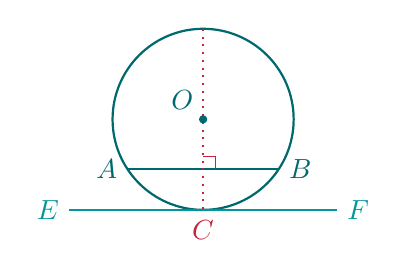
\begin{tikzpicture}[scale=1]
    \draw[thick, color=brandNavy] (0,0) circle (1.15);
    \coordinate (O) at (0,0);
    \coordinate (C) at (0,-1.15);
    \coordinate (A) at (-0.962,-0.63);
    \coordinate (B) at (0.962,-0.63);
    \draw[thick, color=brandNavy] (A) node[left] {$A$} -- (B) node[right] {$B$};
    \draw[thick, color=brandBlue] (-1.7,-1.15) node[left] {$E$} -- (1.7,-1.15) node[right] {$F$};
    \draw[thick, dotted, color=brandCrimson] (0,1.15) -- (C) node[below] {$C$};
    \fill[brandNavy] (O) circle (1.5pt) node[above left] {$O$};
    \draw[color=brandCrimson] (0,-0.47) -| (0.16,-0.63);
  \end{tikzpicture}
\end{minipage}
\end{khcard}

\vspace{3pt}
\begin{khcard}
\begin{minipage}[c]{0.65\textwidth}
  \exhead{18} គេឲ្យបន្ទាត់ពីរ $AB$ និង $AC$ ប៉ះរង្វង់ផ្ចិត $O$ ត្រង់ចំណុចរៀង $B$ និង $C$ ។ ស្រាយបំភ្លឺថា ៖
  \begin{itemize}[leftmargin=15pt, itemsep=2pt]
    \item[\alphabadge{ក}] $AB = AC$
    \item[\alphabadge{ខ}] $\angle BAO = \angle OAC$
    \item[\alphabadge{គ}] $\angle BOA = \angle AOC$
    \item[\alphabadge{ឃ}] $\angle OBA = \angle OCA$
  \end{itemize}
\end{minipage}\hfill
\begin{minipage}[c]{0.33\textwidth}
  \centering
  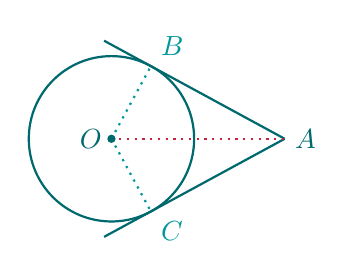
\begin{tikzpicture}[scale=1]
    \draw[thick, color=brandNavy] (0,0) circle (1.05);
    \coordinate (O) at (0,0);
    \coordinate (A) at (2.2,0);
    \coordinate (B) at (61.5:1.05);
    \coordinate (C) at (-61.5:1.05);
    \draw[thick, color=brandNavy] ($(B)!-0.35!(A)$) -- (A) node[right] {$A$};
    \draw[thick, color=brandNavy] ($(C)!-0.35!(A)$) -- (A);
    \draw[thick, dotted, color=brandCrimson] (O) -- (A);
    \draw[thick, dotted, color=brandBlue] (O) -- (B) node[above right] {$B$};
    \draw[thick, dotted, color=brandBlue] (O) -- (C) node[below right] {$C$};
    \fill[brandNavy] (O) circle (1.5pt) node[left] {$O$};
  \end{tikzpicture}
\end{minipage}
\end{khcard}

\vspace{3pt}
\begin{khboxmagenta}
  \begin{minipage}[c]{0.68\textwidth}
    បើបន្ទាត់ពីរគូសចេញពីចំណុចរួមមួយនៅក្រៅរង្វង់ហើយប៉ះរង្វង់នេះត្រង់ចំណុច $B$ និង $C$ គេបាន
    \begin{enumerate}[label=\protect\secbadge{\arabic*}, leftmargin=15pt, itemsep=2pt, topsep=1pt]
      \item បន្ទាត់ប៉ះនៃរង្វង់កែងទៅនឹងកាំត្រង់ចំណុចប៉ះ $\angle OBA = \angle OCA = 90^\circ$
      \item បន្ទាត់ប៉ះពីរទៅនឹងរង្វង់ដែលគូសចេញពីចំណុចរួមមួយនៅក្រៅរង្វង់មានប្រវែងស្មើគ្នា $AB = AC$
      \item បន្ទាត់ដែលគូសចេញពីចំណុចក្រៅរង្វង់មុំឈមទៅផ្ចិតនៃរង្វង់ ជាកន្លះបន្ទាត់ពុះនៃមុំឈមដែលផ្គុំដោយបន្ទាត់ប៉ះទាំងពីរ និងមុំដែលផ្គុំដោយកាំនៃរង្វង់ ៖
      \begin{itemize}[leftmargin=10pt, itemsep=1pt]
        \item $\angle OAB = \angle OAC$
        \item $\angle COA = \angle BOA$
      \end{itemize}
    \end{enumerate}
  \end{minipage}\hfill
  \begin{minipage}[c]{0.28\textwidth}
    \centering
    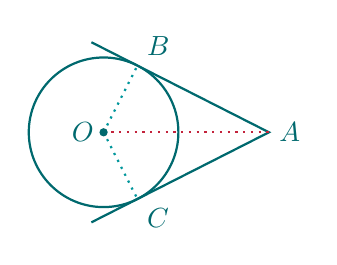
\begin{tikzpicture}[scale=1]
      \draw[thick, color=brandNavy] (0,0) circle (0.95);
      \coordinate (O) at (0,0);
      \coordinate (A) at (2.1,0);
      \coordinate (B) at (63.1:0.95);
      \coordinate (C) at (-63.1:0.95);
      \draw[thick, color=brandNavy] ($(B)!-0.35!(A)$) -- (A) node[right] {$A$} -- ($(C)!-0.35!(A)$);
      \node[above right, color=brandNavy] at (B) {$B$};
      \node[below right, color=brandNavy] at (C) {$C$};
      \draw[thick, dotted, color=brandCrimson] (O) -- (A);
      \draw[thick, dotted, color=brandBlue] (O) -- (B);
      \draw[thick, dotted, color=brandBlue] (O) -- (C);
      \fill[brandNavy] (O) circle (1.5pt) node[left] {$O$};
    \end{tikzpicture}
  \end{minipage}
\end{khboxmagenta}

\vspace{4pt}
\begin{multicols}{2}
  \noindent
  \exhead{19} $PA$ និង $PB$ ជាបន្ទាត់ប៉ះទៅនឹងរង្វង់ផ្ចិត $O$ ត្រង់ចំណុច $A$ និង $B$ (ដូចរូបខាងស្ដាំ) ៖ បើ $\angle ABP = 65^\circ$ ៖
  \begin{itemize}[leftmargin=15pt, itemsep=1.5pt]
    \item[\alphabadge{ក}] គណនាមុំ $\angle AOB$
    \item[\alphabadge{ខ}] គណនាមុំ $\angle AOP$
  \end{itemize}
  \begin{center}
    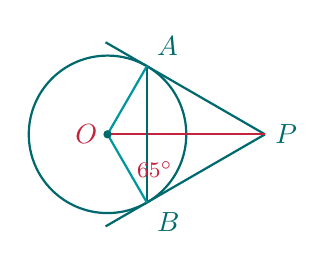
\begin{tikzpicture}[scale=1]
      \draw[thick, color=brandNavy] (0,0) circle (1.0);
      \coordinate (O) at (0,0);
      \coordinate (P) at (2.0,0);
      \coordinate (A) at (60:1.0);
      \coordinate (B) at (-60:1.0);
      \draw[thick, color=brandNavy] ($(A)!-0.35!(P)$) -- (P) node[right] {$P$};
      \draw[thick, color=brandNavy] ($(B)!-0.35!(P)$) -- (P);
      \draw[thick, color=brandCrimson] (O) node[left] {$O$} -- (P);
      \draw[thick, color=brandNavy] (A) node[above right] {$A$} -- (B) node[below right] {$B$};
      \draw[thick, color=brandBlue] (O) -- (A);
      \draw[thick, color=brandBlue] (O) -- (B);
      \node[color=brandCrimson] at (0.6, -0.45) {\footnotesize $65^\circ$};
      \fill[brandNavy] (O) circle (1.5pt);
    \end{tikzpicture}
  \end{center}

  \columnbreak

  \noindent
  \exhead{20} $TA$ និង $TB$ ជាបន្ទាត់ប៉ះទៅនឹងរង្វង់ផ្ចិត $O$ ដែលមានកាំស្មើនឹង $5\text{cm}$ ៖ បើ $\angle ATB = 60^\circ$ ចូរគណនា ៖
  \begin{itemize}[leftmargin=15pt, itemsep=1.5pt]
    \item[\alphabadge{ក}] $\angle AOB$
    \item[\alphabadge{ខ}] ផ្ទៃក្រឡានៃចម្រៀកថាសតូច $AOB$ $\left(\pi = \frac{22}{7}\right)$
  \end{itemize}
  \begin{center}
    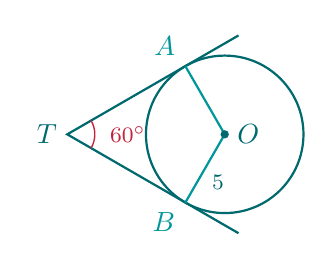
\begin{tikzpicture}[scale=1]
      \draw[thick, color=brandNavy] (0,0) circle (1.0);
      \coordinate (O) at (0,0);
      \coordinate (T) at (-2.0,0);
      \coordinate (A) at (120:1.0);
      \coordinate (B) at (-120:1.0);
      \draw[thick, color=brandNavy] ($(A)!-0.45!(T)$) -- (T) node[left] {$T$} -- ($(B)!-0.45!(T)$);
      \draw[thick, color=brandBlue] (O) -- (A) node[above left] {$A$};
      \draw[thick, color=brandBlue] (O) -- (B) node[below left] {$B$};
      \fill[brandNavy] (O) circle (1.5pt) node[right=1pt] {$O$};
      \draw[color=brandCrimson, line width=0.5pt] ($(T)+(30:0.35)$) arc (30:-30:0.35);
      \node[right=2pt, color=brandCrimson] at ($(T)+(0:0.35)$) {\footnotesize $60^\circ$};
      \node[below right=-1pt, color=brandNavy] at ($(O)!0.5!(B)$) {\footnotesize $5$};
    \end{tikzpicture}
  \end{center}
\end{multicols}

\vspace{4pt}
\begin{multicols}{2}
  \noindent
  \exhead{21} នៅក្នុងរូបខាងស្ដាំនេះមាន $O$ ជាផ្ចិតនៃរង្វង់ហើយ $PA$ និង $PB$ ជាបន្ទាត់ប៉ះទៅនឹងរង្វង់រៀងគ្នាតត្រង់ $A$ និង $B$ រង្វាស់គិតជា $\text{cm}$ ៖ ចូរគណនា
  \begin{itemize}[leftmargin=15pt, itemsep=1.5pt]
    \item[\alphabadge{ក}] រង្វាស់ $b$
    \item[\alphabadge{ខ}] រង្វាស់ $c$
    \item[\alphabadge{គ}] បរិមាត្រនៃចតុកោណ $OAPB$
    \item[\alphabadge{ឃ}] ផ្ទៃក្រឡានៃចតុកោណ $OAPB$
  \end{itemize}
  \begin{center}
    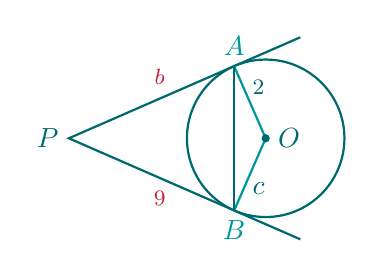
\begin{tikzpicture}[scale=1]
      \draw[thick, color=brandNavy] (0,0) circle (1.0);
      \coordinate (O) at (0,0);
      \coordinate (P) at (-2.5,0);
      \coordinate (A) at (113.6:1.0);
      \coordinate (B) at (-113.6:1.0);
      \draw[thick, color=brandNavy] ($(A)!-0.4!(P)$) -- (P) node[left] {$P$} -- ($(B)!-0.4!(P)$);
      \draw[thick, color=brandBlue] (O) -- (A) node[above] {$A$};
      \draw[thick, color=brandBlue] (O) -- (B) node[below] {$B$};
      \draw[thick, color=brandNavy] (A) -- (B);
      \fill[brandNavy] (O) circle (1.5pt) node[right=1pt] {$O$};
      \node[above, color=brandCrimson] at ($(P)!0.55!(A)+(0,0.05)$) {\footnotesize $b$};
      \node[below, color=brandCrimson] at ($(P)!0.55!(B)+(0,-0.05)$) {\footnotesize $9$};
      \node[above right=-2pt, color=brandNavy] at ($(O)!0.55!(A)$) {\footnotesize $2$};
      \node[below right=-2pt, color=brandNavy] at ($(O)!0.55!(B)$) { $c$};
    \end{tikzpicture}
  \end{center}

  \columnbreak

  \noindent
  \exhead{22} គេមាន $PA$ និង $PB$ ជាបន្ទាត់ប៉ះទៅនឹងរង្វង់ដែលមានផ្ចិត $O$ និងកាំ $3\text{cm}$ ៖ គេឲ្យ $AP = 82.4\text{cm}$ និង $\angle AOB = 140^\circ$ ៖ ចូរគណនាផ្ទៃក្រឡានៃ
  \begin{itemize}[leftmargin=15pt, itemsep=1.5pt]
    \item[\alphabadge{ក}] ចតុកោណ $APBO$
    \item[\alphabadge{ខ}] ចម្រៀកថាសតូច $AOB$ យក $\left(\pi = \frac{22}{7}\right)$
  \end{itemize}
  \begin{center}
    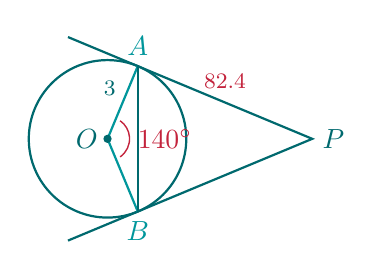
\begin{tikzpicture}[scale=1]
      \draw[thick, color=brandNavy] (0,0) circle (1.0);
      \coordinate (O) at (0,0);
      \coordinate (P) at (2.6,0);
      \coordinate (A) at (67.4:1.0);
      \coordinate (B) at (-67.4:1.0);
      \draw[thick, color=brandNavy] ($(A)!-0.4!(P)$) -- (P) node[right] {$P$} -- ($(B)!-0.4!(P)$);
      \draw[thick, color=brandBlue] (O) -- (A) node[above] {$A$};
      \draw[thick, color=brandBlue] (O) -- (B) node[below] {$B$};
      \draw[thick, color=brandNavy] (A) -- (B);
      \fill[brandNavy] (O) circle (1.5pt) node[left] {$O$};
      \node[above, color=brandCrimson] at ($(A)!0.5!(P)+(0,0.05)$) {\footnotesize $82.4$};
      \node[above left=-1pt, color=brandNavy] at ($(O)!0.5!(A)$) {\footnotesize $3$};
      \draw[color=brandCrimson, line width=0.5pt] (-55:0.28) arc (-55:55:0.28);
      \node[right, color=brandCrimson] at (0.26,0) { $140^\circ$};
    \end{tikzpicture}
  \end{center}
\end{multicols}

\vspace{3pt}
\begin{multicols}{2}
  \noindent
  \exhead{23} ក្នុងរង្វង់ផ្ចិត $O$ គេមាន $AT$ និង $BT$ មានប្រវែង $20\text{cm}$ ៖ បើ $TQO$ ជាបន្ទាត់ត្រង់ដែល $TQ = 10\text{cm}$ ៖ ចូររករង្វាស់នៃកាំរង្វង់ ៖
  \begin{center}
    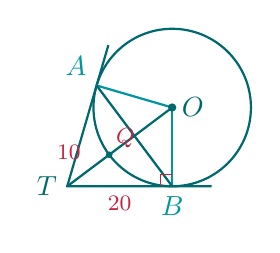
\begin{tikzpicture}[scale=1]
      \draw[thick, color=brandNavy] (0,0) circle (1.0);
      \coordinate (O) at (0,0);
      \coordinate (B) at (0,-1.0);
      \coordinate (T) at (-1.333,-1.0);
      \coordinate (A) at (-0.96, 0.28);
      \coordinate (Q) at (-0.8, -0.6);
      \draw[thick, color=brandNavy] ($(A)!-0.4!(T)$) -- (T) node[left] {$T$} -- (0.5,-1.0);
      \draw[thick, color=brandNavy] (T) -- (O);
      \draw[thick, color=brandBlue] (O) -- (A) node[above left] {$A$};
      \draw[thick, color=brandBlue] (O) -- (B) node[below] {$B$};
      \draw[thick, color=brandNavy] (A) -- (B);
      \fill[brandNavy] (O) circle (1.5pt) node[right] {$O$};
      \fill[brandNavy] (Q) circle (1.2pt);
      \node[above right=-1pt, color=brandCrimson] at (Q) {\footnotesize $Q$};
      \node[above left, color=brandCrimson] at ($(T)!0.55!(Q)$) {\footnotesize $10$};
      \node[below, color=brandCrimson] at ($(T)!0.5!(B)$) {\footnotesize $20$};
      \draw[color=brandCrimson, line width=0.5pt] (0,-0.85) -| (-0.15,-1.0);
    \end{tikzpicture}
  \end{center}

  \columnbreak

  \noindent
  \exhead{24} នៅក្នុងរង្វង់ផ្ចិត $O$ ដែលមានកាំ $4.5\text{cm}$ ៖ គេមាន $TA$ និង $TB$ ជាបន្ទាត់ប៉ះនឹងរង្វង់រៀងគ្នាតត្រង់ $A$ និង $B$ ដែល $TA = 9\text{cm}$ ៖
  \begin{itemize}[leftmargin=15pt, itemsep=1.5pt]
    \item[\alphabadge{ក}] គណនាបរិមាត្រនៃចតុកោណ $OATB$
    \item[\alphabadge{ខ}] គណនាផ្ទៃក្រឡានៃចតុកោណ $OATB$
  \end{itemize}
  \begin{center}
    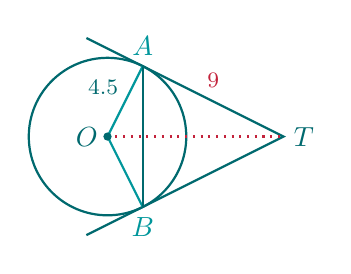
\begin{tikzpicture}[scale=1]
      \draw[thick, color=brandNavy] (0,0) circle (1.0);
      \coordinate (O) at (0,0);
      \coordinate (T) at (2.236,0);
      \coordinate (A) at (63.43:1.0);
      \coordinate (B) at (-63.43:1.0);
      \draw[thick, color=brandNavy] ($(A)!-0.4!(T)$) -- (T) node[right] {$T$} -- ($(B)!-0.4!(T)$);
      \draw[thick, color=brandBlue] (O) -- (A) node[above] {$A$};
      \draw[thick, color=brandBlue] (O) -- (B) node[below] {$B$};
      \draw[thick, color=brandNavy] (A) -- (B);
      \draw[thick, dotted, color=brandCrimson] (O) -- (T);
      \fill[brandNavy] (O) circle (1.5pt) node[left] {$O$};
      \node[above, color=brandCrimson] at ($(A)!0.5!(T)+(0,0.05)$) {\footnotesize $9$};
      \node[above left=-1pt, color=brandNavy] at ($(O)!0.5!(A)$) {\footnotesize $4.5$};
    \end{tikzpicture}
  \end{center}
\end{multicols}

\vspace{3pt}
\begin{multicols}{2}
  \noindent
  \exhead{25} $TA$ និង $TB$ ជាបន្ទាត់ប៉ះទៅនឹងរង្វង់ផ្ចិត $O$ ដែលមានកាំ $9\text{cm}$ ។ បើ $\angle ATB = 110^\circ$ ។ ចូរគណនា
  \begin{itemize}[leftmargin=15pt, itemsep=1.5pt]
    \item[\alphabadge{ក}] $\angle AOB$
    \item[\alphabadge{ខ}] ផ្ទៃក្រឡាចម្រៀកថាសតូច $AOB$ ដែល $\pi = \frac{22}{7}$
  \end{itemize}
  \begin{center}
    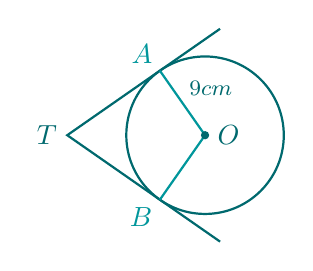
\begin{tikzpicture}[scale=1]
      \draw[thick, color=brandNavy] (0,0) circle (1.0);
      \coordinate (O) at (0,0);
      \coordinate (T) at (-1.75,0);
      \coordinate (A) at (125:1.0);
      \coordinate (B) at (-125:1.0);
      \draw[thick, color=brandNavy] ($(T)!1.65!(A)$) -- (T) node[left] {$T$} -- ($(T)!1.65!(B)$);
      \draw[thick, color=brandBlue] (O) -- (A) node[above left=-1pt] {$A$};
      \draw[thick, color=brandBlue] (O) -- (B) node[below left=-1pt] {$B$};
      \fill[brandNavy] (O) circle (1.5pt) node[right=1pt] {$O$};
      \node[above right=-1pt, color=brandNavy] at ($(O)!0.5!(A)$) {\footnotesize $9\text{cm}$};
    \end{tikzpicture}
  \end{center}

  \columnbreak

  \noindent
  \exhead{26} $ST$ និង $RT$ ជាបន្ទាត់ប៉ះទៅនឹងរង្វង់មួយមានផ្ចិត $O$ ដែល $ST = RT = 20\text{cm}$ ។ បើ $TQO$ ជាបន្ទាត់ត្រង់មួយដែល $TQ = 10\text{cm}$ ។ ចូរគណនាកាំនៃរង្វង់ $OQ$ ៖
  \vspace{6pt}
  \begin{center}
    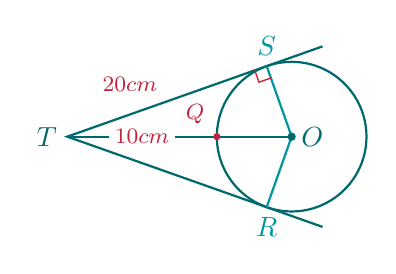
\begin{tikzpicture}[scale=1]
      \draw[thick, color=brandNavy] (0,0) circle (0.95);
      \coordinate (O) at (0,0);
      \coordinate (T) at (-2.85,0);
      \coordinate (S) at (109.5:0.95);
      \coordinate (R) at (-109.5:0.95);
      \coordinate (Q) at (-0.95,0);
      \draw[thick, color=brandNavy] ($(T)!1.28!(S)$) -- (T) node[left] {$T$} -- ($(T)!1.28!(R)$);
      \draw[thick, color=brandNavy] (T) -- (O);
      \draw[thick, color=brandBlue] (O) -- (S) node[above] {$S$};
      \draw[thick, color=brandBlue] (O) -- (R) node[below] {$R$};
      \fill[brandNavy] (O) circle (1.5pt) node[right] {$O$};
      \fill[brandCrimson] (Q) circle (1.3pt);
      \node[above left=1pt, color=brandCrimson] at (Q) {\footnotesize $Q$};
      \node[above left, color=brandCrimson] at ($(T)!0.5!(S)$) {\footnotesize $20\text{cm}$};
      \node[fill=white, inner sep=2pt, text=brandCrimson] at ($(T)!0.5!(Q)$) {\footnotesize $10\text{cm}$};
      \coordinate (S1) at ($(S)!0.16cm!(T)$);
      \coordinate (S2) at ($(S)!0.16cm!(O)$);
      \draw[color=brandCrimson, line width=0.5pt] (S1) -- ($ (S1) + (S2) - (S) $) -- (S2);
    \end{tikzpicture}
  \end{center}
\end{multicols}

\vspace{2pt}
\noindent
\exhead{27} ក្នុងរូបនីមួយៗខាងក្រោមនេះ គេមាន $PT$ និង $PV$ ជាបន្ទាត់ប៉ះទៅនឹងរង្វង់ផ្ចិត $O$ ត្រង់ $T$ និង $V$ ។ រករង្វាស់មុំដែលមិនស្គាល់ ៖
\vspace{2pt}
\begin{center}
  \begin{minipage}[t]{0.24\textwidth}
    \centering
    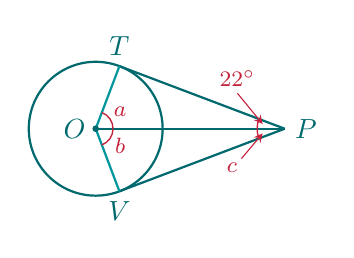
\begin{tikzpicture}[scale=1]
      \coordinate (O) at (0,0);
      \coordinate (P) at (2.4,0);
      \draw[thick, color=brandNavy] (O) circle (0.85);
      \coordinate (T) at (69.26:0.85);
      \coordinate (V) at (-69.26:0.85);
      \draw[thick, color=brandNavy] (P) node[right] {$P$} -- (T) node[above] {$T$};
      \draw[thick, color=brandNavy] (P) -- (V) node[below] {$V$};
      \draw[thick, color=brandNavy] (O) node[left] {$O$} -- (P);
      \draw[thick, color=brandBlue] (O) -- (T);
      \draw[thick, color=brandBlue] (O) -- (V);
      \fill[brandNavy] (O) circle (1.2pt);
      \draw[color=brandCrimson, line width=0.5pt] (0.22,0) arc (0:69.26:0.22);
      \node[color=brandCrimson] at (35:0.38) {\footnotesize $a$};
      \draw[color=brandCrimson, line width=0.5pt] (0.22,0) arc (0:-69.26:0.22);
      \node[color=brandCrimson] at (-35:0.38) {\footnotesize $b$};
      \draw[color=brandCrimson, line width=0.5pt] ($(P)+(-0.35,0)$) arc (180:159.26:0.35);
      \draw[color=brandCrimson, line width=0.5pt] ($(P)+(-0.35,0)$) arc (180:200.74:0.35);
      \draw[->, >=stealth, color=brandCrimson, line width=0.4pt] ($(P)+(-0.6,0.45)$) node[above=-1pt] {\footnotesize $22^\circ$} -- ($(P)+(-0.28,0.06)$);
      \draw[->, >=stealth, color=brandCrimson, line width=0.4pt] ($(P)+(-0.55,-0.38)$) node[below left=-2pt] {\footnotesize $c$} -- ($(P)+(-0.28,-0.06)$);
    \end{tikzpicture}\\[1pt]
    \textbf{\color{brandNavy}(ក)}
  \end{minipage}\hfill
  \begin{minipage}[t]{0.24\textwidth}
    \centering
    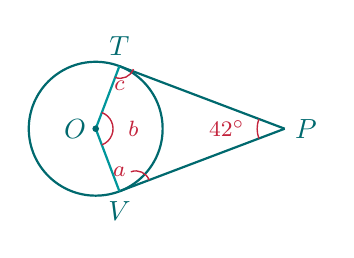
\begin{tikzpicture}[scale=1]
      \coordinate (O) at (0,0);
      \coordinate (P) at (2.4,0);
      \draw[thick, color=brandNavy] (O) circle (0.85);
      \coordinate (T) at (69.26:0.85);
      \coordinate (V) at (-69.26:0.85);
      \draw[thick, color=brandNavy] (P) node[right] {$P$} -- (T) node[above] {$T$};
      \draw[thick, color=brandNavy] (P) -- (V) node[below] {$V$};
      \draw[thick, color=brandBlue] (O) -- (T);
      \draw[thick, color=brandBlue] (O) -- (V);
      \fill[brandNavy] (O) circle (1.2pt) node[left] {$O$};
      \draw[color=brandCrimson, line width=0.5pt] ($(P)+(-0.35,0)$) arc (180:159.26:0.35);
      \draw[color=brandCrimson, line width=0.5pt] ($(P)+(-0.35,0)$) arc (180:200.74:0.35);
      \node[left=1pt, color=brandCrimson] at ($(P)+(-0.35,0)$) {\footnotesize $42^\circ$};
      \draw[color=brandCrimson, line width=0.5pt] (69.26:0.22) arc (69.26:-69.26:0.22);
      \node[right=2pt, color=brandCrimson] at (0.22,0) {\footnotesize $b$};
      \draw[color=brandCrimson, line width=0.5pt] ($(T)!0.18!(O)$) arc (249.26:339.26:0.18);
      \node[below=2pt, color=brandCrimson] at (T) {\footnotesize $c$};
      \draw[color=brandCrimson, line width=0.5pt] ($(V)!0.18!(P)$) arc (20.74:110.74:0.18);
      \node[above=2pt, color=brandCrimson] at (V) {\footnotesize $a$};
    \end{tikzpicture}\\[1pt]
    \textbf{\color{brandNavy}(ខ)}
  \end{minipage}\hfill
  \begin{minipage}[t]{0.24\textwidth}
    \centering
    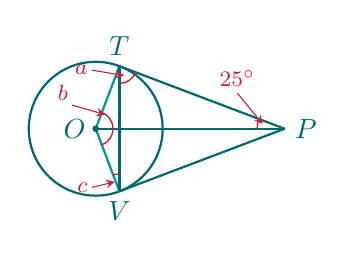
\begin{tikzpicture}[scale=1]
      \coordinate (O) at (0,0);
      \coordinate (P) at (2.4,0);
      \draw[thick, color=brandNavy] (O) circle (0.85);
      \coordinate (T) at (69.26:0.85);
      \coordinate (V) at (-69.26:0.85);
      \draw[thick, color=brandNavy] (P) node[right] {$P$} -- (T) node[above] {$T$};
      \draw[thick, color=brandNavy] (P) -- (V) node[below] {$V$};
      \draw[thick, color=brandNavy] (O) node[left] {$O$} -- (P);
      \draw[thick, color=brandBlue] (O) -- (T);
      \draw[thick, color=brandBlue] (O) -- (V);
      \draw[thick, color=brandNavy] (T) -- (V);
      \fill[brandNavy] (O) circle (1.2pt);
      \draw[color=brandCrimson, line width=0.5pt] ($(P)+(-0.35,0)$) arc (180:159.26:0.35);
      \draw[->, >=stealth, color=brandCrimson, line width=0.4pt] ($(P)+(-0.6,0.45)$) node[above=-1pt] {\footnotesize $25^\circ$} -- ($(P)+(-0.28,0.06)$);
      \draw[color=brandCrimson, line width=0.5pt] (69.26:0.22) arc (69.26:0:0.22);
      \draw[color=brandCrimson, line width=0.5pt] (0:0.22) arc (0:-69.26:0.22);
      \draw[->, >=stealth, color=brandCrimson, line width=0.4pt] ($(O)+(-0.3,0.3)$) node[above left=-2pt] {\footnotesize $b$} -- ($(O)+(0.12,0.18)$);
      \draw[color=brandCrimson, line width=0.5pt] ($(T)+(0,-0.22)$) arc (270:339.26:0.22);
      \draw[->, >=stealth, color=brandCrimson, line width=0.4pt] ($(T)+(-0.35,-0.05)$) node[left=-2pt] {\footnotesize $a$} -- ($(T)+(0.06,-0.12)$);
      \draw[color=brandCrimson, line width=0.5pt] ($(V)+(0,0.22)$) arc (90:110.74:0.22);
      \draw[->, >=stealth, color=brandCrimson, line width=0.4pt] ($(V)+(-0.35,0.05)$) node[left=-2pt] {\footnotesize $c$} -- ($(V)+(-0.06,0.12)$);
    \end{tikzpicture}\\[1pt]
    \textbf{\color{brandNavy}(គ)}
  \end{minipage}\hfill
  \begin{minipage}[t]{0.24\textwidth}
    \centering
    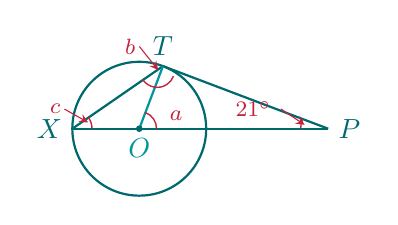
\begin{tikzpicture}[scale=1]
      \coordinate (O) at (0,0);
      \coordinate (X) at (-0.85,0);
      \coordinate (P) at (2.4,0);
      \draw[thick, color=brandNavy] (O) circle (0.85);
      \coordinate (T) at (69.26:0.85);
      \draw[thick, color=brandNavy] (P) node[right] {$P$} -- (T) node[above] {$T$};
      \draw[thick, color=brandNavy] (X) node[left] {$X$} -- (P);
      \draw[thick, color=brandNavy] (X) -- (T);
      \draw[thick, color=brandBlue] (O) node[below] {$O$} -- (T);
      \fill[brandNavy] (O) circle (1.2pt);
      \draw[color=brandCrimson, line width=0.5pt] ($(P)+(-0.35,0)$) arc (180:159.26:0.35);
      \draw[->, >=stealth, color=brandCrimson, line width=0.4pt] ($(P)+(-0.6,0.25)$) node[left] {\footnotesize $21^\circ$} -- ($(P)+(-0.3,0.05)$);
      \draw[color=brandCrimson, line width=0.5pt] (0.22,0) arc (0:69.26:0.22);
      \node[right=1pt, color=brandCrimson] at (35:0.28) {\footnotesize $a$};
      \draw[color=brandCrimson, line width=0.5pt] ($(X)+(0.25,0)$) arc (0:34.63:0.25);
      \draw[->, >=stealth, color=brandCrimson, line width=0.4pt] ($(X)+(-0.1,0.25)$) node[left=-2pt] {\footnotesize $c$} -- ($(X)+(0.2,0.08)$);
      \draw[color=brandCrimson, line width=0.5pt] ($(T)!0.22!(X)$) arc (214.63:339.26:0.22);
      \draw[->, >=stealth, color=brandCrimson, line width=0.4pt] ($(T)+(-0.3,0.25)$) node[left=-2pt] {\footnotesize $b$} -- ($(T)+(-0.06,-0.05)$);
    \end{tikzpicture}\\[1pt]
    \textbf{\color{brandNavy}(ឃ)}
  \end{minipage}
\end{center}

\newpage
% -------------------------------------------------------------------------
% CIRCUMSCRIBED QUADRILATERALS

\khsection{៤}{អនុវត្តន៍លក្ខណៈជ្រុងឈមនៃចតុកោណចារឹកក្រៅរង្វង់}

\vspace{1pt}
\begin{khcard}
\begin{minipage}[c]{0.68\textwidth}
  \exhead{28} នៅក្នុងចតុកោណ $ABCD$ ដូចរូបខាងស្ដាំ\\
  ជ្រុងទាំងបួនជាបន្ទាត់ប៉ះរង្វង់ត្រង់ $P, Q, R$ និង $S$ បង្ហាញថា
  \begin{itemize}[leftmargin=15pt, itemsep=0pt, topsep=1pt]
    \item[\alphabadge{ក}] $AP = AS, BP = BQ, CQ = CR$ និង $DR = DS$
    \item[\alphabadge{ខ}] $AB + CD = AD + BC$
  \end{itemize}
\end{minipage}\hfill
\begin{minipage}[c]{0.30\textwidth}
  \centering
  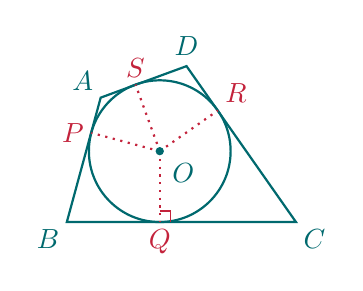
\begin{tikzpicture}[scale=1]
    \coordinate (O) at (0,0);
    \draw[thick, color=brandNavy] (O) circle (0.90);
    
    % Tangent points on circle
    \coordinate (P) at (165:0.90);
    \coordinate (Q) at (270:0.90);
    \coordinate (R) at (35:0.90);
    \coordinate (S) at (110:0.90);
    
    % Tangent line intersection vertices (tangential quadrilateral ABCD)
    \coordinate (A) at (-0.75, 0.68);
    \coordinate (B) at (-1.18, -0.90);
    \coordinate (C) at (1.73, -0.90);
    \coordinate (D) at (0.34, 1.08);
    
    \draw[thick, color=brandNavy] (A) node[above left=-1pt] {$A$} -- (D) node[above] {$D$} -- (C) node[below right=-1pt] {$C$} -- (B) node[below left=-1pt] {$B$} -- cycle;
    
    \draw[thick, dotted, color=brandCrimson] (O) -- (P) node[left=-1pt] {$P$};
    \draw[thick, dotted, color=brandCrimson] (O) -- (Q) node[below=-1pt] {$Q$};
    \draw[thick, dotted, color=brandCrimson] (O) -- (R) node[above right=-1pt] {$R$};
    \draw[thick, dotted, color=brandCrimson] (O) -- (S) node[above=-1pt] {$S$};
    \fill[brandNavy] (O) circle (1.5pt) node[below right=1pt] {$O$};
    \draw[color=brandCrimson, line width=0.5pt] (0, -0.76) -| (0.14, -0.90);
  \end{tikzpicture}
\end{minipage}


\centerline{\textbf{\fontsize{9.5}{9.5}\selectfont\color{brandCrimson}\kml ស្រាយបញ្ជាក់ ៖}}
\vspace{1pt}
\noindent
\textbf{\alphabadge{ក} }បង្ហាញថា $AP = AS, BP = BQ, CQ = CR$ និង $DR = DS$ ៖\\
តាមលក្ខណៈបន្ទាត់ប៉ះគូសចេញពីចំណុចតែមួយមកកាន់រង្វង់ គេបាន ៖
\begin{itemize}[leftmargin=12pt, itemsep=0pt, parsep=0pt, topsep=1pt]
  \item $AS$ និង $AP$ ប៉ះត្រង់ $S$ និង $P$ គូសពី $A \implies AS = AP$ \quad $\bullet$ $BP$ និង $BQ$ ប៉ះត្រង់ $P$ និង $Q$ គូសពី $B \implies BP = BQ$
  \item $CQ$ និង $CR$ ប៉ះត្រង់ $Q$ និង $R$ គូសពី $C \implies CQ = CR$ \quad $\bullet$ $DS$ និង $DR$ ប៉ះត្រង់ $S$ និង $R$ គូសពី $D \implies DS = DR$
\end{itemize}

\vspace{1pt}
\noindent
\textbf{\alphabadge{ខ}} បង្ហាញថា $AB + CD = AD + BC$ ៖\\
\indent គេមាន $AB = AP + PB$ , $CD = CR + RD$ , $AD = AS + SD$ , $BC = BQ + QC$\\
\indent ដូចនេះ $\begin{aligned}[t]
  AB + CD &= (AP + PB) + (CR + RD) = AS + BQ + QC + SD\\
  &= (AS + SD) + (BQ + QC) = AD + BC
\end{aligned}$\\
\indent ដូចនេះ \textbf{$AB + CD = AD + BC$}\hfill\ding{111}
\end{khcard}
\vspace{-2pt}
\begin{khboxmagenta}
  \textbf{ក្នុងចតុកោណចារឹកក្រៅរង្វង់ ផលបូករង្វាស់ជ្រុងឈមមានរង្វាស់ស្មើគ្នា ៖}
 {\large\color{brandCrimson}\textbf{$AB + CD = AD + BC$}}
\end{khboxmagenta}

\vspace{2pt}
\setlength{\columnsep}{18pt}
\setlength{\columnseprule}{0.5pt}
\def\columnseprulecolor{\color{cardBorder}}

\begin{multicols}{2}
  \noindent
  \exhead{29} រង្វង់ផ្ចិត $O$ ប៉ះនឹងជ្រុងទាំងបួននៃចតុកោណ $ABCD$ ដែល $AB = 20\text{cm}, CD = 14\text{cm}$ និង $BC = 11\text{cm}$ ៖ គណនារង្វាស់ $AD$ ៖\par

  {\centering
    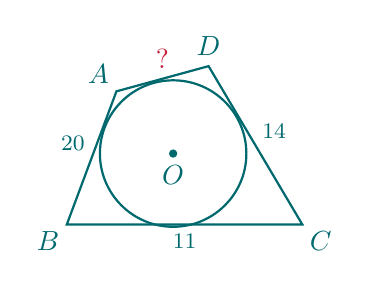
\begin{tikzpicture}[scale=1]
      \coordinate (O) at (0,0);
      \draw[thick, color=brandNavy] (O) circle (0.93);
      \coordinate (A) at (-0.72, 0.79);
      \coordinate (B) at (-1.35, -0.90);
      \coordinate (C) at (1.64, -0.90);
      \coordinate (D) at (0.45, 1.11);
      \draw[thick, color=brandNavy] (A) node[above left=-1pt] {$A$} -- (D) node[above=0pt] {$D$} -- (C) node[below right=-1pt] {$C$} -- (B) node[below left=-1pt] {$B$} -- cycle;
      \fill[brandNavy] (O) circle (1.5pt) node[below=1pt] {$O$};
      \node[above, color=brandCrimson] at ($(A)!0.5!(D)$) {$?$};
      \node[above left=-1pt, color=brandNavy] at ($(A)!0.5!(B)$) {\footnotesize $20$};
      \node[below, color=brandNavy] at ($(B)!0.5!(C)$) {\footnotesize $11$};
      \node[above right=-1pt, color=brandNavy] at ($(C)!0.5!(D)$) {\footnotesize $14$};
    \end{tikzpicture}\par}

  \vspace{3pt}
  \noindent
  \exhead{30} ក្នុងរូបខាងក្រោមនេះ $ABC$ ជាត្រីកោណសមបាតដែលមានកំពូល $A$ ៖ ចូរស្រាយបំភ្លឺថា $BR = RC$ ៖\par
  \vspace{1pt}
  {\centering
    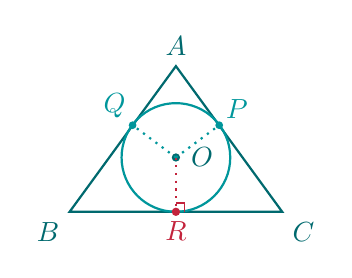
\begin{tikzpicture}[scale=1]
      \coordinate (A) at (0, 1.85);
      \coordinate (B) at (-1.35, 0);
      \coordinate (C) at (1.35, 0);
      \draw[thick, color=brandNavy] (A) node[above] {$A$} -- (B) node[below left] {$B$} -- (C) node[below right] {$C$} -- cycle;
      \draw[thick, color=brandTeal] (0, 0.69) circle (0.69);
      \fill[brandCrimson] (0,0) circle (1.5pt) node[below, color=brandCrimson] {$R$};
      \fill[brandTeal] (0.55, 1.1) circle (1.4pt) node[above right=-1pt, color=brandTeal] {$P$};
      \fill[brandTeal] (-0.55, 1.1) circle (1.4pt) node[above left=-1pt, color=brandTeal] {$Q$};
      \fill[brandNavy] (0, 0.69) circle (1.5pt) node[right=2pt] {$O$};
      \draw[thick, dotted, color=brandCrimson] (0, 0.69) -- (0,0);
      \draw[thick, dotted, color=brandTeal] (0, 0.69) -- (0.55, 1.1);
      \draw[thick, dotted, color=brandTeal] (0, 0.69) -- (-0.55, 1.1);
      \draw[color=brandCrimson, line width=0.5pt] (0, 0.11) -| (0.11, 0);
    \end{tikzpicture}\par}

  \vspace{2pt}
  \noindent
  \exhead{31} រង្វង់ពីរមានផ្ចិតរួម $O$ មានកាំ $8\text{cm}$ និង $10\text{cm}$ ៖ $AB$ ជាអង្កត់ធ្នូនៃរង្វង់ធំហើយប៉ះរង្វង់តូចត្រង់ $T$ ៖ ចូរគណនា $AB$ ៖\par
  \vspace{1pt}
  {\centering
    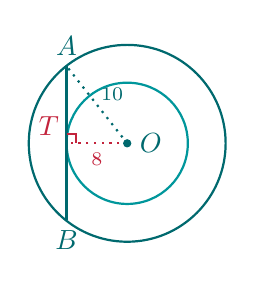
\begin{tikzpicture}[scale=1]
      \draw[thick, color=brandNavy] (0,0) circle (1.25);
      \draw[thick, color=brandBlue] (0,0) circle (0.77);
      \coordinate (O) at (0,0);
      \coordinate (T) at (-0.77,0);
      \coordinate (A) at (-0.77, 0.98);
      \coordinate (B) at (-0.77, -0.98);
      \draw[thick, color=brandNavy] (A) node[above] {$A$} -- (B) node[below] {$B$};
      \draw[thick, dotted, color=brandCrimson] (O) -- (T) node[above left=-1pt, color=brandCrimson] {$T$};
      \draw[thick, dotted, color=brandNavy] (O) -- (A);
      \fill[brandNavy] (O) circle (1.5pt) node[right=1pt] {$O$};
      \draw[color=brandCrimson, line width=0.5pt] (-0.77, 0.12) -| (-0.65, 0);
      \node[below, color=brandCrimson] at ($(O)!0.5!(T)$) {\scriptsize $8$};
      \node[above right=-2pt, color=brandNavy] at ($(O)!0.5!(A)$) {\scriptsize $10$};
    \end{tikzpicture}\par}

  \columnbreak

  \noindent
  \exhead{32} ក្នុងរូបខាងក្រោមនេះ ចតុកោណព្នាយសមបាត $ABCD$ ($AB \parallel CD$) ចារឹកក្រៅរង្វង់ផ្ចិត $O$ មានបាត $AB = 4\text{cm}$ និង $CD = 16\text{cm}$ ៖ ចូរគណនាប្រវែង $AD$ និង $BC$ ៖\\
  %(\textbf{ណែនាំ} ៖ ប្រើលក្ខណៈ $AB + CD = AD + BC$ ដោយ $AD = BC$)\par
\vspace{-0.2cm}
  {\centering
    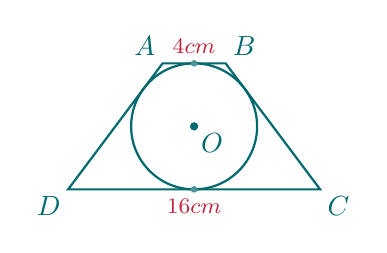
\begin{tikzpicture}[scale=1]
      \coordinate (O) at (0,0);
      \draw[thick, color=brandNavy] (O) circle (0.80);
      \coordinate (A) at (-0.40, 0.80);
      \coordinate (B) at (0.40, 0.80);
      \coordinate (C) at (1.60, -0.80);
      \coordinate (D) at (-1.60, -0.80);
      \draw[thick, color=brandNavy] (A) node[above left=-1pt] {$A$} -- (B) node[above right=-1pt] {$B$} -- (C) node[below right=-1pt] {$C$} -- (D) node[below left=-1pt] {$D$} -- cycle;
      \fill[brandNavy] (O) circle (1.5pt) node[below right=-1pt] {$O$};
      \node[above, color=brandCrimson] at ($(A)!0.5!(B)$) {\footnotesize $4\text{cm}$};
      \node[below, color=brandCrimson] at ($(D)!0.5!(C)$) {\footnotesize $16\text{cm}$};
      \fill[brandNavy!70] (0, 0.80) circle (1.2pt);
      \fill[brandNavy!70] (0, -0.80) circle (1.2pt);
    \end{tikzpicture}\par}
\vspace{-0.2cm}
  \noindent
  \exhead{33} ក្នុងរូបខាងក្រោម ចតុកោណ $ABCD$ ចារឹកក្រៅរង្វង់ផ្ចិត $O$ មានរង្វាស់ជ្រុង $AB = 2x - 1, CD = 3x + 4, BC = x + 6$ និង $AD = 17\text{cm}$ ៖ ចូរគណនាតម្លៃនៃ $x$ និងប្រវែងជ្រុង $AB, CD, BC$ ៖\par
  \vspace{1pt}
  {\centering
    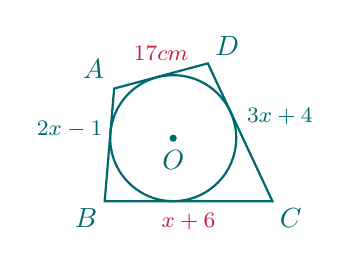
\begin{tikzpicture}[scale=1]
      \coordinate (O) at (0,0);
      \draw[thick, color=brandNavy] (O) circle (0.80);
      \coordinate (A) at (-0.75, 0.63);
      \coordinate (B) at (-0.87, -0.80);
      \coordinate (C) at (1.26, -0.80);
      \coordinate (D) at (0.44, 0.95);
      \draw[thick, color=brandNavy] (A) node[above left=0pt] {$A$} -- (D) node[above right=-1pt] {$D$} -- (C) node[below right=-1pt] {$C$} -- (B) node[below left=-1pt] {$B$} -- cycle;
      \fill[brandNavy] (O) circle (1.3pt) node[below=1pt] {$O$};
      \node[above left=-1pt, color=brandNavy] at ($(A)!0.5!(B)$) {\footnotesize $2x-1$};
      \node[above right=-1pt, color=brandNavy] at ($(C)!0.5!(D)$) {\footnotesize $3x+4$};
      \node[above=2pt, color=brandCrimson] at ($(A)!0.5!(D)$) {\footnotesize $17\text{cm}$};
      \node[below=1pt, color=brandCrimson] at ($(B)!0.5!(C)$) {\footnotesize $x+6$};
    \end{tikzpicture}\par}
\vspace{-0.2cm}
  \noindent
  \exhead{34} ក្នុងរូបខាងក្រោម ចតុកោណ $ABCD$ ចារឹកក្រៅរង្វង់ផ្ចិត $O$ មានរង្វាស់ជ្រុង $AB = 3x - 2, CD = 2x + 5, BC = 2x + 1$ និង $AD = 14\text{cm}$ ៖ ចូរគណនាតម្លៃនៃ $x$ និងប្រវែងជ្រុង $AB, CD, BC$ ៖\par
\vspace{-0.2cm}
  {\centering
    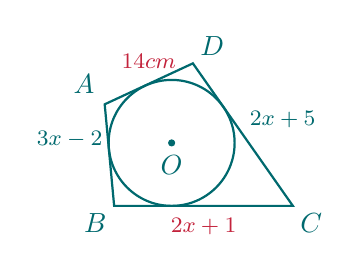
\begin{tikzpicture}[scale=1]
      \coordinate (O) at (0,0);
      \draw[thick, color=brandNavy] (O) circle (0.80);
      \coordinate (A) at (-0.85, 0.49);
      \coordinate (B) at (-0.73, -0.80);
      \coordinate (C) at (1.54, -0.80);
      \coordinate (D) at (0.27, 1.01);
      \draw[thick, color=brandNavy] (A) node[above left=0pt] {$A$} -- (D) node[above right=-1pt] {$D$} -- (C) node[below right=-1pt] {$C$} -- (B) node[below left=-1pt] {$B$} -- cycle;
      \fill[brandNavy] (O) circle (1.3pt) node[below=1pt] {$O$};
      \node[above left=-1pt, color=brandNavy] at ($(A)!0.5!(B)$) {\footnotesize $3x-2$};
      \node[above right=-1pt, color=brandNavy] at ($(C)!0.5!(D)$) {\footnotesize $2x+5$};
      \node[above=2pt, color=brandCrimson] at ($(A)!0.5!(D)$) {\footnotesize $14\text{cm}$};
      \node[below=1pt, color=brandCrimson] at ($(B)!0.5!(C)$) {\footnotesize $2x+1$};
    \end{tikzpicture}\par}
\end{multicols}

\newpage
% -------------------------------------------------------------------------
% RELATIVE POSITIONS OF TWO CIRCLES

\khsection{៥}{ទីតាំងរង្វង់}

គេមានរង្វង់ពីរដែលមានផ្ចិត $O$ និង $O'$ និងកាំរៀងគ្នា $r$ និង $r'$ ។ ហើយ $d$ ជាចម្ងាយរវាងផ្ចិតទាំងពីរ ដូចរូបខាងក្រោម ៖

\vspace{4pt}
% 5 Cases Grid in clean cards
\begin{minipage}[t]{0.48\textwidth}
  \begin{khcard}
    \centering
    \secbadge{1} \textcolor{brandCrimson}{\textbf{$d > r + r'$}}\\[2pt]
    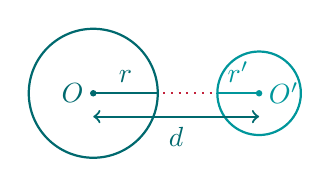
\begin{tikzpicture}[scale=0.78]
      \draw[thick, color=brandNavy] (0,0) circle (1.05);
      \draw[thick, color=brandBlue] (2.7,0) circle (0.68);
      \coordinate (O) at (0,0);
      \coordinate (O1) at (2.7,0);
      \draw[thick, dotted, color=brandCrimson] (O) -- (O1);
      \draw[<->, thick, color=brandNavy] (0,-0.38) -- (2.7,-0.38) node[midway, below] {$d$};
      \draw[thick, color=brandNavy] (O) -- ++(1.05,0) node[midway, above] {$r$};
      \draw[thick, color=brandBlue] (O1) -- ++(-0.68,0) node[midway, above] {$r'$};
      \fill[brandNavy] (O) circle (1.5pt) node[left] {$O$};
      \fill[brandBlue] (O1) circle (1.5pt) node[right] {$O'$};
    \end{tikzpicture}\\[2pt]
    \textbf{\color{brandNavy}រង្វង់គ្មានចំណុចរួម}
  \end{khcard}
\end{minipage}\hfill
\begin{minipage}[t]{0.48\textwidth}
  \begin{khcard}
    \centering
    \secbadge{2} \textcolor{brandCrimson}{\textbf{$d = r + r'$}}\\[2pt]
    \begin{tikzpicture}[scale=0.78]
      \draw[thick, color=brandNavy] (0,0) circle (0.95);
      \draw[thick, color=brandBlue] (1.65,0) circle (0.68);
      \coordinate (O) at (0,0);
      \coordinate (O1) at (1.65,0);
      \draw[thick, color=brandCrimson] (O) -- (O1);
      \draw[<->, thick, color=brandNavy] (0,-0.38) -- (1.65,-0.38) node[midway, below] {$d$};
      \node[above, color=brandNavy] at (0.48,0) {$r$};
      \node[above, color=brandBlue] at (1.3,0) {$r'$};
      \fill[brandNavy] (O) circle (1.5pt) node[left] {$O$};
      \fill[brandBlue] (O1) circle (1.5pt) node[right] {$O'$};
    \end{tikzpicture}\\[2pt]
    \textbf{\color{brandNavy}រង្វង់មានចំណុចរួមមួយ (ប៉ះក្រៅ)}
  \end{khcard}
\end{minipage}

\vspace{4pt}
\begin{minipage}[t]{0.32\textwidth}
  \begin{khcard}
    \centering
    \secbadge{3} \textcolor{brandCrimson}{\textbf{\footnotesize $r-r' < d < r+r'$}}\\[2pt]
    \begin{tikzpicture}[scale=1]
      \draw[thick, color=brandNavy] (0,0) circle (1.05);
      \draw[thick, color=brandBlue] (1.15,0) circle (0.76);
      \coordinate (O) at (0,0);
      \coordinate (O1) at (1.15,0);
      \coordinate (P) at (0.58,0.85);
      \draw[thick, color=brandNavy] (O) -- (P) node[midway, left] {$r$};
      \draw[thick, color=brandBlue] (O1) -- (P) node[midway, right] {$r'$};
      \draw[<->, thick, color=brandCrimson] (0,-0.38) -- (1.15,-0.38) node[midway, below] {$d$};
      \fill[brandNavy] (O) circle (1.5pt) node[left] {$O$};
      \fill[brandBlue] (O1) circle (1.5pt) node[right] {$O'$};
    \end{tikzpicture}\\[2pt]
    \textbf{\footnotesize\color{brandNavy} រង្វង់កាត់គ្នាពីរចំណុច}
  \end{khcard}
\end{minipage}\hfill
\begin{minipage}[t]{0.32\textwidth}
  \begin{khcard}
    \centering
    \secbadge{4} \textcolor{brandCrimson}{\textbf{$d = r - r'$}}\\[2pt]
    \begin{tikzpicture}[scale=0.85]
      \draw[thick, color=brandNavy] (0,0) circle (1.15);
      \draw[thick, color=brandBlue] (0.48,0) circle (0.67);
      \coordinate (O) at (0,0);
      \coordinate (O1) at (0.48,0);
      \draw[thick, dotted, color=brandNavy] (O) -- (1.15,0);
      \draw[<->, thick, color=brandNavy] (0,0.28) -- (1.15,0.28) node[midway, above] {$r$};
      \draw[<->, thick, color=brandBlue] (0.48,-0.2) -- (1.15,-0.2) node[midway, below] {$r'$};
      \draw[<->, thick, color=brandCrimson] (0.3,0) -- ++(-0.55,-0.55) node[midway, below ] {$d$};
      \fill[brandNavy] (O) circle (1.5pt) node[below] {$O$};
      \fill[brandBlue] (O1) circle (1.5pt) node[below] {$O'$};
    \end{tikzpicture}\\[2pt]
    \textbf{\footnotesize\color{brandNavy} រង្វង់ប៉ះក្នុង}
  \end{khcard}
\end{minipage}\hfill
\begin{minipage}[t]{0.32\textwidth}
  \begin{khcard}
    \centering
    \secbadge{5} \textcolor{brandCrimson}{\textbf{$d < r - r'$}}\\[2pt]
    \begin{tikzpicture}[scale=0.9]
      \draw[thick, color=brandNavy] (0,0) circle (1.15);
      \draw[thick, color=brandBlue] (0.28,0) circle (0.48);
      \coordinate (O) at (0,0);
      \coordinate (O1) at (0.28,0);
      \draw[<->, thick, color=brandNavy] (0,0.28) -- (1.15,0.28) node[midway, above] {$r$};
      \draw[<->, thick, color=brandBlue] (0.28,-0.15) -- (0.76,-0.15) node[midway, below] {$r'$};
      \draw[<->, thick, color=brandCrimson] (0.2,0) -- ++(-0.38,-0.38) node[midway, below left] {$d$};
      \fill[brandNavy] (O) circle (1.5pt) node[below] {$O$};
      \fill[brandBlue] (O1) circle (1.5pt) node[below] {$O'$};
    \end{tikzpicture}\\[2pt]
    \textbf{\footnotesize\color{brandNavy} រង្វង់គ្មានចំណុចរួម}
  \end{khcard}
\end{minipage}

\setlength{\columnsep}{18pt}
\setlength{\columnseprule}{0.5pt}
\def\columnseprulecolor{\color{cardBorder}}

\begin{multicols}{2}
  \noindent
  \exhead{35} គេឲ្យរង្វង់ពីរដែលមានកាំរៀងគ្នា $r = 5\text{cm}, r' = 3\text{cm}$ ហើយ $OO'$ ជាចម្ងាយរវាងផ្ចិតទាំងពីរ ដែល $OO' = 2x + 1$ ៖ ចូរកំណត់ $x$ ដើម្បីឲ្យ ៖
  \begin{itemize}[leftmargin=15pt, itemsep=1.5pt, topsep=2pt]
    \item[\alphabadge{ក}] រង្វង់ទាំងពីរប៉ះក្រៅ
    \item[\alphabadge{ខ}] រង្វង់ទាំងពីរប៉ះក្នុង
    \item[\alphabadge{គ}] រង្វង់កាត់គ្នាត្រង់ពីរចំណុច
  \end{itemize}

  \vspace{5pt}
  \noindent
  \exhead{36} គេឲ្យរង្វង់ពីរដែលមានកាំរៀងគ្នា $r = 5\text{cm}$ និង $r' = 3\text{cm}$ ៖ $OO'$ កាត់រង្វង់រៀងគ្នាត្រង់ចំណុច $A$ និង $B$ ៖ ចូរគណនាប្រវែង $AB$ ៖\par
  \vspace{3pt}
  {\centering
    \begin{tikzpicture}[scale=1]
      \draw[thick, color=brandNavy] (0,0) circle (1.00);
      \draw[thick, color=brandBlue] (2.65,0) circle (0.65);
      \coordinate (O) at (0,0);
      \coordinate (O1) at (2.65,0);
      \coordinate (A) at (1.00,0);
      \coordinate (B) at (2.00,0);
      \draw[thick, color=brandNavy] (O) -- (A);
      \draw[thick, dotted, color=brandCrimson] (A) -- (B);
      \draw[thick, color=brandBlue] (B) -- (O1);
      \fill[brandNavy] (O) circle (1.4pt) node[left] {\scriptsize $O$};
      \fill[brandBlue] (O1) circle (1.4pt) node[right] {\scriptsize $O'$};
      \node[below=1.5pt, color=brandNavy] at (0.50,0) {\scriptsize $r$};
      \node[above=1.5pt, color=brandCrimson] at (A) {\scriptsize $A$};
      \node[above=1.5pt, color=brandCrimson] at (B) {\scriptsize $B$};
      \node[below=1.5pt, color=brandBlue] at (2.32,0) {\scriptsize $r'$};
    \end{tikzpicture}\par}

  \columnbreak

  \noindent
  \exhead{37} គេឲ្យរង្វង់ពីរដែលមានកាំរៀងគ្នា $r = 7\text{cm}, r' = 3\text{cm}$ ហើយ $OO'$ ជាចម្ងាយរវាងផ្ចិតទាំងពីរ ដែល $OO' = 2x + 2$ ៖ ចូរកំណត់ $x$ ដើម្បីឲ្យ ៖
  \begin{itemize}[leftmargin=15pt, itemsep=1.5pt, topsep=2pt]
    \item[\alphabadge{ក}] រង្វង់ទាំងពីរប៉ះក្រៅ
    \item[\alphabadge{ខ}] រង្វង់ទាំងពីរប៉ះក្នុង
    \item[\alphabadge{គ}] រង្វង់កាត់គ្នាត្រង់ពីរចំណុច
  \end{itemize}

  \vspace{5pt}
  \noindent
  \exhead{38} គេឲ្យរង្វង់ពីរដែលមានកាំរៀងគ្នា $r = 6\text{cm}, r' = 4\text{cm}$ ហើយ $OO'$ ជាចម្ងាយរវាងផ្ចិតទាំងពីរ ដែល $OO' = 4x - 2$ ៖ ចូរកំណត់ $x$ ដើម្បីឲ្យ ៖
  \begin{itemize}[leftmargin=15pt, itemsep=1.5pt, topsep=2pt]
    \item[\alphabadge{ក}] រង្វង់ទាំងពីរប៉ះក្រៅ
    \item[\alphabadge{ខ}] រង្វង់ទាំងពីរប៉ះក្នុង
    \item[\alphabadge{គ}] រង្វង់កាត់គ្នាត្រង់ពីរចំណុច
  \end{itemize}
\end{multicols}

% -------------------------------------------------------------------------
% COMMON TANGENTS

\khsection{៦}{បន្ទាត់ប៉ះរួម}

បន្ទាត់ប៉ះរួមនៃរង្វង់ពីរផ្សេងគ្នាអាស្រ័យលើទំនាក់ទំនងទីតាំងនៃរង្វង់ទាំងពីរដូចរូបខាងក្រោម ៖

\vspace{2pt}
\begin{khcard}
\textbf{\fontsize{9.5}{9.5}\selectfont\kml\color{brandNavy} ក. រង្វង់គ្មានចំណុចរួម}

\vspace{0.5pt}
\begin{minipage}[c]{0.66\textwidth}
  \begin{itemize}[leftmargin=11pt, itemsep=1pt, topsep=1pt, parsep=0pt]
    \item[\color{brandBlue}\textbullet] រង្វង់ទាំងពីរគ្មានចំណុចរួម $AB$ និង $CD$ ហៅថា\textbf{\color{brandCrimson}បន្ទាត់ប៉ះរួមខាងក្រៅ} ។ រង្វង់ទាំងពីរស្ថិតនៅតែម្ខាងនៃបន្ទាត់ $AB$ និង $CD$ ។
  \end{itemize}
\end{minipage}\hfill
\begin{minipage}[c]{0.32\textwidth}
  \centering
  \begin{tikzpicture}[scale=1]
    \draw[thick, color=brandNavy] (0,0) circle (0.60);
    \draw[thick, color=brandBlue] (2.2,0) circle (0.80);
    \coordinate (O) at (0,0);
    \coordinate (O1) at (2.2,0);
    \draw[thick, color=brandCrimson] (-0.55, 0.55) node[above left=-1pt] {$C$} -- (2.7, 0.84) node[above right=-1pt] {$D$};
    \draw[thick, color=brandCrimson] (-0.55, -0.55) node[below left=-1pt] {$A$} -- (2.7, -0.84) node[below right=-1pt] {$B$};
    \draw[thick, dotted, color=brandNavy] (O) -- (-0.055, 0.598);
    \draw[thick, dotted, color=brandNavy] (O) -- (-0.055, -0.598);
    \draw[thick, dotted, color=brandBlue] (O1) -- (2.128, 0.797);
    \draw[thick, dotted, color=brandBlue] (O1) -- (2.128, -0.797);
    \fill[brandNavy] (O) circle (1.3pt) node[right=1pt] {$O$};
    \fill[brandBlue] (O1) circle (1.3pt) node[right=1pt] {$O'$};
  \end{tikzpicture}
\end{minipage}

\vspace{-0.2cm}
\begin{minipage}[c]{0.66\textwidth}
  \begin{itemize}[leftmargin=11pt, itemsep=1pt, topsep=1pt, parsep=0pt]
    \item[\color{brandBlue}\textbullet] រង្វង់ទាំងពីរគ្មានចំណុចរួម បន្ទាត់ $MN$ និង $PQ$ ហៅថា\textbf{\color{brandCrimson}បន្ទាត់ប៉ះរួមខាងក្នុង} ។ រង្វង់ទាំងពីរស្ថិតនៅសងខាងនៃបន្ទាត់ $MN$ និង $PQ$ ។
  \end{itemize}
\end{minipage}\hfill
\begin{minipage}[c]{0.32\textwidth}
  \centering
  \begin{tikzpicture}[scale=1]
    \draw[thick, color=brandNavy] (0,0) circle (0.60);
    \draw[thick, color=brandBlue] (2.2,0) circle (0.80);
    \coordinate (O) at (0,0);
    \coordinate (O1) at (2.2,0);
    \draw[thick, color=brandCrimson] (0.02, -0.76) node[below left=-2pt] {$M$} -- (2.05, 0.92) node[above right=-2pt] {$N$};
    \draw[thick, color=brandCrimson] (0.02, 0.76) node[above left=-2pt] {$P$} -- (2.05, -0.92) node[below right=-2pt] {$Q$};
    \draw[thick, dotted, color=brandNavy] (O) -- (0.385, -0.460);
    \draw[thick, dotted, color=brandNavy] (O) -- (0.385, 0.460);
    \draw[thick, dotted, color=brandBlue] (O1) -- (1.687, 0.615);
    \draw[thick, dotted, color=brandBlue] (O1) -- (1.687, -0.615);
    \fill[brandNavy] (O) circle (1.3pt) node[left=1pt] {$O$};
    \fill[brandBlue] (O1) circle (1.3pt) node[right=1pt] {$O'$};
  \end{tikzpicture}
\end{minipage}
\end{khcard}

\vspace{1.5pt}
\begin{khcard}
\textbf{\fontsize{9.5}{9.5}\selectfont\kml\color{brandNavy} ខ. រង្វង់ប៉ះគ្នា}

\vspace{0.5pt}
\begin{minipage}[c]{0.66\textwidth}
  \begin{itemize}[leftmargin=11pt, itemsep=1pt, topsep=1pt, parsep=0pt]
    \item[\color{brandBlue}\textbullet] រង្វង់ពីរមានចំណុចរួមមួយ ហៅថារង្វង់ប៉ះគ្នា ។ $l$ ជាបន្ទាត់ប៉ះរួមដែលរង្វង់ទាំងពីរ ស្ថិតនៅសងខាងនៃបន្ទាត់ $l$ ។
  \end{itemize}
\end{minipage}\hfill
\vspace{-0.2cm}
\begin{minipage}[c]{0.32\textwidth}
  \centering
  \begin{tikzpicture}[scale=1.2]
    \draw[thick, color=brandNavy] (0,0) circle (0.62);
    \draw[thick, color=brandBlue] (1.42,0) circle (0.80);
    \coordinate (O) at (0,0);
    \coordinate (O1) at (1.42,0);
    \draw[thick, color=brandCrimson] (0.62, 1.05) node[above] {$l$} -- (0.62, -1.05);
    \draw[thick, dotted, color=brandNavy] (O) -- (O1);
    \fill[brandNavy] (O) circle (1.3pt) node[left] {$O$};
    \fill[brandBlue] (O1) circle (1.3pt) node[right] {$O'$};
    \fill[brandCrimson] (0.62,0) circle (1.1pt) node[above right] {$A$};
  \end{tikzpicture}
\end{minipage}

\vspace{-0.2cm}
\begin{minipage}[c]{0.66\textwidth}
  \begin{itemize}[leftmargin=11pt, itemsep=1pt, topsep=1pt, parsep=0pt]
    \item[\color{brandBlue}\textbullet] រង្វង់ទាំងពីរមានចំណុចរួមមួយ ។ $l$ ជាបន្ទាត់ប៉ះរួម ។ រង្វង់ទាំងពីរស្ថិតនៅតែម្ខាងនៃបន្ទាត់ $l$ ។
  \end{itemize}
\end{minipage}\hfill
\begin{minipage}[c]{0.32\textwidth}
  \centering
  \begin{tikzpicture}[scale=1.2]
    \draw[thick, color=brandNavy] (0,0) circle (0.95);
    \draw[thick, color=brandBlue] (0.38,0) circle (0.57);
    \coordinate (O) at (0,0);
    \coordinate (O1) at (0.38,0);
    \draw[thick, color=brandCrimson] (0.95, 1.15) node[above] {$l$} -- (0.95, -1.15);
    \draw[thick, dotted, color=brandNavy] (O) -- (0.95,0);
    \fill[brandNavy] (O) circle (1.3pt) node[below] {$O$};
    \fill[brandBlue] (O1) circle (1.3pt) node[below] {$O'$};
  \end{tikzpicture}
\end{minipage}
\end{khcard}

\vspace{1.5pt}
\begin{khcard}[top=2pt, bottom=2pt]
  \textbf{\fontsize{9}{9}\selectfont\kml\color{brandNavy} គ. រង្វង់កាត់គ្នា}
  
  \vspace{0.5pt}
  \begin{minipage}[c]{0.66\textwidth}
    \fontsize{8.5}{11}\selectfont
    រង្វង់ទាំងពីរកាត់គ្នាត្រង់ពីរចំណុច ។ បន្ទាត់ $XY$ និង $ZE$ ជាបន្ទាត់ប៉ះរួមខាងក្រៅ ។
  \end{minipage}\hfill
  \begin{minipage}[c]{0.32\textwidth}
    \centering
    \begin{tikzpicture}[scale=1.2]
      \draw[thick, color=brandNavy] (0,0) circle (0.58);
      \draw[thick, color=brandBlue] (0.85,0) circle (0.70);
      \coordinate (O) at (0,0);
      \coordinate (O1) at (0.85,0);
      \draw[thick, color=brandCrimson] (-0.48, 0.52) node[above left=-2pt] {$X$} -- (1.18, 0.75) node[above right=-2pt] {$Y$};
      \draw[thick, color=brandCrimson] (-0.48, -0.52) node[below left=-2pt] {$Z$} -- (1.18, -0.75) node[below right=-2pt] {$E$};
      \fill[brandNavy] (O) circle (1.2pt) node[left] {$O$};
      \fill[brandBlue] (O1) circle (1.2pt) node[right] {$O'$};
    \end{tikzpicture}
  \end{minipage}
\end{khcard}

\vspace{1.5pt}
\begin{khcard}[top=2pt, bottom=2pt]
  \textbf{\fontsize{9}{9}\selectfont\kml\color{brandNavy} ឃ. រង្វង់តូចនៅក្នុងរង្វង់ធំ}
  
  \vspace{0.5pt}
  \begin{minipage}[c]{0.66\textwidth}
    \fontsize{8.5}{11}\selectfont
    គ្មានចំណុចប៉ះរួម ។
  \end{minipage}\hfill
  \begin{minipage}[c]{0.32\textwidth}
    \centering
    \begin{tikzpicture}[scale=1.3]
      \draw[thick, color=brandNavy] (0,0) circle (0.88);
      \draw[thick, color=brandBlue] (0.42,0.05) circle (0.42);
      \fill[brandNavy] (0,0) circle (1.2pt) node[left=1pt] {$O$};
      \fill[brandBlue] (0.42,0.05) circle (1.2pt) node[right=1pt] {$O'$};
    \end{tikzpicture}
  \end{minipage}
\end{khcard}

\vspace{2pt}
\setlength{\columnsep}{16pt}
\setlength{\columnseprule}{0.5pt}
\def\columnseprulecolor{\color{cardBorder}}

\begin{multicols}{2}
  % Column 1: Exercise 39 & Exercise 41
  \noindent
  \exhead{39} គេមានរង្វង់ពីរផ្សេងគ្នាដែលមានរង្វាស់កាំ $a$ និង $b$ គិតជា $\text{cm}$ ហើយចម្ងាយរវាងផ្ចិតទាំងពីរស្មើ $d$ ៖ ចូររកចំនួនបន្ទាត់ប៉ះរួមតាមករណីខាងក្រោម ៖\par
  \vspace{1.5pt}
  {\centering
  \renewcommand{\arraystretch}{1.12}
  \footnotesize
  \begin{tabular}{|p{1.8cm}|c|c|c|c|}
    \hline
    \rowcolor{brandLightBlue}
    & \textbf{\color{brandNavy} ក} & \textbf{\color{brandNavy} ខ} & \textbf{\color{brandNavy} គ} & \textbf{\color{brandNavy} ឃ} \\
    \hline
    \centering $a$ & $3$ & $4$ & $2$ & $5$ \\
    \hline
    \centering $b$ & $5$ & $3$ & $3$ & $3$ \\
    \hline
    \centering $d$ & $10$ & $6$ & $5$ & $2$ \\
    \hline
    \centering \textbf{\color{brandCrimson} បន្ទាត់ប៉ះ} & & & & \\
    \hline
  \end{tabular}\par}

  \vspace{4pt}
  \noindent
  \exhead{41} គេមាន $MA, MB$ និង $MC$ ជាបន្ទាត់ប៉ះទៅនឹងរង្វង់ផ្ចិត $O$ និងផ្ចិត $O'$ ៖ ចូរបង្ហាញថា $MA = MC$ ៖\par
  \vspace{2pt}
  {\centering
  \begin{tikzpicture}[scale=1.2]
    \coordinate (O) at (-0.80, 0);
    \coordinate (O1) at (1.00, 0);
    \coordinate (B) at (0, 0);
    \coordinate (M) at (0, 1.45);
    \coordinate (A) at (-1.246, 0.655);
    \coordinate (C) at (1.354, 0.935);
    \draw[thick, color=brandNavy] (O) circle (0.80);
    \draw[thick, color=brandBlue] (O1) circle (1.00);
    \draw[thick, color=brandNavy] (M) -- (-1.53, 0.47);
    \draw[thick, color=brandNavy] (M) -- (1.68, 0.81);
    \draw[thick, color=brandCrimson] (0, 1.55) -- (0, -0.45);
    \fill[brandNavy] (O) circle (1.3pt) node[below] {$O$};
    \fill[brandBlue] (O1) circle (1.3pt) node[below] {$O'$};
    \fill[brandCrimson] (B) circle (1.2pt) node[below right=-1pt] {$B$};
    \node[above] at (M) {$M$};
    \node[above left=-2pt, color=brandNavy] at (A) {$A$};
    \node[above right=-2pt, color=brandNavy] at (C) {$C$};
  \end{tikzpicture}\par}

  \columnbreak

  % Column 2: Exercise 40 & Exercise 42
  \noindent
  \exhead{40} $XY$ ជាបន្ទាត់ប៉ះរួមខាងក្នុងរង្វង់ផ្ចិត $O$ និង $O'$ ៖ $XS$ ជាបន្ទាត់ប៉ះរង្វង់ផ្ចិត $O$ ត្រង់ $S$ ហើយ $YT$ ជាបន្ទាត់ប៉ះរង្វង់ផ្ចិត $O'$ ត្រង់ $T$ ៖ ចូរបង្ហាញថា $XS = YT$ ៖\par
  \vspace{2pt}
  {\centering
  \begin{tikzpicture}[scale=1.2]
    \coordinate (O) at (0, 0);
    \coordinate (O1) at (2.05, 0);
    \coordinate (Y) at (0.580, -0.621);
    \coordinate (X) at (1.674, 0.402);
    \coordinate (S) at (0.236, 0.817);
    \coordinate (T) at (2.076, -0.549);
    \draw[thick, color=brandNavy] (O) circle (0.85);
    \draw[thick, color=brandBlue] (O1) circle (0.55);
    % Internal tangent line XY
    \draw[thick, color=brandCrimson] (0.20, -0.98) -- (2.05, 0.76);
    % Tangent line XS
    \draw[thick, color=brandNavy] (X) -- (-0.30, 0.97);
    % Tangent line YT
    \draw[thick, color=brandNavy] (Y) -- (2.65, -0.52);
    % Dotted radii
    \draw[thick, dotted, color=brandNavy] (O) -- (S);
    \draw[thick, dotted, color=brandNavy] (O) -- (Y);
    \draw[thick, dotted, color=brandBlue] (O1) -- (X);
    \draw[thick, dotted, color=brandBlue] (O1) -- (T);
    % Points and labels
    \fill[brandNavy] (O) circle (1.3pt) node[left] {$O$};
    \fill[brandBlue] (O1) circle (1.3pt) node[right] {$O'$};
    \fill[brandNavy] (S) circle (1.1pt) node[above] {$S$};
    \fill[brandBlue] (T) circle (1.1pt) node[below] {$T$};
    \fill[brandCrimson] (X) circle (1.1pt) node[above left=-2pt] {$X$};
    \fill[brandCrimson] (Y) circle (1.1pt) node[below right=-2pt] {$Y$};
  \end{tikzpicture}\par}

  \vspace{4pt}
  \noindent
  \exhead{42} គេមានរង្វង់ពីរមានទំហំខុសគ្នាដែលមានផ្ចិត $O$ និង $O'$ ៖ រង្វង់ទាំងពីរនេះមានបន្ទាត់ប៉ះរួមមួយ ដែលមានចម្ងាយរវាងផ្ចិតទាំងពីរស្មើនឹង $4\text{cm}$ និងមានចម្ងាយរវាងផ្ចិត $1\text{cm}$ ដូចរូបខាងក្រោម ៖ ចូរគណនាកាំនៃរង្វង់ទាំងពីរ ៖\par
  \vspace{2pt}
  {\centering
  \begin{tikzpicture}[scale=1.2]
    \draw[thick, color=brandNavy] (0,0) circle (0.90);
    \draw[thick, color=brandBlue] (1.65,0) circle (0.75);
    \coordinate (O) at (0,0);
    \coordinate (O1) at (1.65,0);
    \draw[thick, color=brandCrimson] (O) -- (O1);
    \draw[<->, thick, color=brandNavy] (0,-0.30) -- (1.65,-0.30) node[midway, below] {$4$};
    \fill[brandNavy] (O) circle (1.3pt) node[left] {$O$};
    \fill[brandBlue] (O1) circle (1.3pt) node[right] {$O'$};
  \end{tikzpicture}\hspace{0.5cm}%
  \begin{tikzpicture}[scale=1.2]
    \draw[thick, color=brandNavy] (0,0) circle (0.95);
    \draw[thick, color=brandBlue] (0.38,0) circle (0.57);
    \coordinate (O) at (0,0);
    \coordinate (O1) at (0.38,0);
    \draw[thick, color=brandNavy] (O) -- (0.38,0);
    \draw[<->, thick, color=brandCrimson] (0,0.20) -- (0.38,0.20) node[midway, above] {$1$};
    \fill[brandNavy] (O) circle (1.3pt) node[below] {$O$};
    \fill[brandBlue] (O1) circle (1.3pt) node[below] {$O'$};
  \end{tikzpicture}\par}
\end{multicols}



\end{document}
